\documentclass{brandeis-dissertation3.14}

\usepackage{amsmath}
\usepackage{amssymb}
\usepackage{hyperref}
\usepackage{cleveref}
\usepackage[sorting=none]{biblatex}
\usepackage{graphicx}
\usepackage{subfig}
\usepackage{color}
\usepackage{xspace}
\usepackage{tabularx}\usepackage{calc}\usepackage{array}
\usepackage{lscape}
\usepackage{multirow}
\usepackage{verbatim}
\usepackage{Dissertation_Addepalli-defs}

\renewcommand\thechapter{\Roman{chapter}}
\renewcommand\thesection{\arabic{section}}
%\renewcommand{\numberline}[1]{Chapter #1 }
%\renewcommand\thesubsection{(\alph{subsection})}

\addbibresource{Dissertation_Addepalli.bib}

\title{Search for Long Lived Heavy Neutral Leptons in Events with Displaced Vertices in ATLAS }
\author{Sagar Vidya Addepalli}
\graduationmonth{May}
\graduationyear{2024}
\program{Department of Physics}
\advisor{Gabriella Sciolla}
\signoff{Wendy Cadge}{Dean}
\committee{Prof. Gabriella Sciolla, Department of Physics, Brandeis University\\
Prof. Aram Apyan, Department of Physics, Brandeis University\\
Dr. Maximilian Emanuel Goblirsch-Kolb, European Organization for Nuclear Research}


\begin{document}

\maketitlepage
\makeapproval
\frontmatter

\begin{dissertation-acknowledgements}
I want to thank me, for believing in me and working hard.
\end{dissertation-acknowledgements}
\addcontentsline{toc}{section}{Acknowledgements}

\begin{dissertation-abstract}
Lorem ipsum dolor sit amet, consectetur adipiscing elit, sed do eiusmod tempor incididunt ut labore et dolore magna aliqua. Ut enim ad minim veniam, quis nostrud exercitation ullamco laboris nisi ut aliquip ex ea commodo consequat. Duis aute irure dolor in reprehenderit in voluptate velit esse cillum dolore eu fugiat nulla pariatur. Excepteur sint occaecat cupidatat non proident, sunt in culpa qui officia deserunt mollit anim id est laborum.
\end{dissertation-abstract}
\addcontentsline{toc}{section}{Abstract}

\doublespacing

\tableofcontents{}

\clearpage

\listoftables
\addcontentsline{toc}{section}{List of Tables}
\pagebreak
\listoffigures
\addcontentsline{toc}{section}{List of Figures}
\pagebreak
\setcounter{secnumdepth}{0}
\chapter*{List of Abbreviations}
\addcontentsline{toc}{section}{List of Abbreviations}
\begin{itemize}
    \item ATLAS: A Toroidal LHC ApparatuS
    \item BSM: Beyond Standard Model
    \item CMS: Compact Muon Solenoid
    \item CSC: Cathode Strip Chamber
    \item ECAL: Electromagnetic Calorimeter
    \item HCAL: Hadronic Calorimeter
    \item HNL: Heavy Neutral Lepton
    \item ID: Inner Detector
    \item IP: Interaction Point
    \item LHC: Large Hadron Collider
    \item MDT: Monitored Drift Tube
    \item MIP: Minimum Ionizing Particle
    \item MS: Muon System / Muon Spectrometer
    \item $pp$: proton--proton
    \item PV: Primary Vertex
    \item RPC: Resistive Plate Chamber
    \item SM: Standard Model
    \item SV: Secondary Vertex
    \item TGC: Thin Gap Chamber
\end{itemize}
\setcounter{secnumdepth}{2}

\startbody

\chapter{Introduction}
\label{chap:intro}
\vspace{1in}
{\large
``I can thank the fact that I was born at just the right time. A few years older or younger, I would have missed the opportunity... One might call the period from 1925 onward for a few years the Golden Age of Physics when our basic ideas were developing very rapidly and there was plenty of work for everyone to do."

\hfill -Paul Dirac, J. Robert Oppenheimer Memorial Prize Speech, 1969}
\vspace{1in}

The Standard Model (SM) of Particle Physics, in its current form, is the most (or even the only) widely accepted complete theory of the particle nature of the universe. It provides a mathematical description of the three out of four fundamental forces of nature: Electroweak Force, Strong Force, and the Electromagnetic Force. After its full formulation circa 1975, the model has proved to be extremely successful in predicting natural phenomena at the smallest of scales and highest of energies. Despite that, a few but critical open problems challenge the foundations and completeness of the SM, and beg for theoretical extensions beyond the Standard Model (BSM) that can provide solutions to these problems. Chapter~\ref{chap:theory} outlines the fundamental structure of the SM and lists the open problems that plague it. An extension to the SM in the form of long-lived sterile neutrinos is presented which forms the baselines model used in the analysis presented in this dissertation. The apparatus used to test this model is the ATLAS experiment at the Large Hadron Collider, both of which are described in~\cref{chap:experiment}, along with the techniques used to collect data and stitch the electric signatures into individual physical objects such as particles and their decays. The overview of this analysis is presented in~\cref{chap:ana_overview} with the exact goals we have set out to achieve. The various steps of the analysis method and the statistical structure of extracting the strength of the model are detailed in~\cref{chap:ana_strategy}, followed by the results in~\cref{chap:results}.~\Cref{chap:conclusion} summarizes the inferences of this search, explains its limitations, and lists out possible improvements in the future versions of this adventure.

\chapter{Theory}
\label{chap:theory}
This chapter describes the theoretical framework which the analysis presented in the dissertation is based on. The Standard Model (SM) is briefly described in~\cref{sec:sm} along with its limitations in the form of inability to explain observed anomalies.~\Cref{sec:hnl} introduces a family of Beyond Standard Model (BSM) particles, Heavy Neutral Leptons (HNLs), proposed to explain some of these anomalies. HNLs form the benchmark model probed in this search.

\section{Standard Model}\label{sec:sm}
The Standard Model is our best understanding of the particulate nature of the universe at the most fundamental level. The theory\footnote{The description of the Standard Model is adapted from the book ``Quarks and Leptons"~\cite{Halzen:1984mc}, with modified notations for simplicity and self-consistency.} considers of two kinds of particles: \textit{fermions}, which have half-integer spins and hence follow Fermi-Dirac statistics, and \textit{bosons}, which have integer spins and follow Bose-Einstein statistics. 

Fermions make up all the visible matter while gauge bosons act as the mediators of forces of interaction between them.\footnote{except gravity, for which there is no known particle mediator, and the SM gives no description of the nature of gravity.}. The strong force, which is responsible for binding nuclei together, is described by the theoretical framework of Quantum Chromodynamics (QCD) whose mediators are eight \textit{gluons}. The weak force causes radioactive decays to occur mediated by the $W^\pm$ and $Z$ bosons. Lastly, the electromagnetic (EM) interaction is mediated by \textit{photons}. The electromagnetic and weak interactions are explained together by the Electroweak (EW) theory, and are commonly known as the electroweak interaction.

\begin{figure}[!ht]
    \centering
    \includegraphics[width=.8\linewidth]{figures/theory/SM_no_HNL.pdf}
    \caption{The elementary particles in the Standard Model with their mass and electric charge.~\cite{Gninenko2012}}
    \label{fig:sm}
\end{figure}

The particles of the SM are summarized in~\cref{fig:sm} along with their mass and electric charge. The fermions are organized in three generations (two particles per generation) and two families. The first family is quarks, which have non-zero electric and color charges. Since these are quantum numbers for the EM and QCD interactions, quarks participate in both. The three generations of quarks are \textit{up}/\textit{down}, \textit{charm}/\textit{strange}, and \textit{top}/\textit{bottom}, commonly identified as quark flavors where the flavor is designated by the first letter of their names. The second family of fermions is leptons. Each generation of leptons consists a (electrically) charged-neutral pair, where the charged particles participate in the EM interaction while none of them participate in QCD. The charged leptons are \textit{electrons} ($e$), \textit{muons} ($\mu$), and \textit{taus} ($\tau$) each having a neutral partner \textit{neutrino} ($\nu_e,\,\nu_\mu,\,\nu_\tau$). Each fermion has an anti-fermion partner with an indentical mass and magnitude of spin but opposite physical charges. All fermions have non-zero weak isospin quantum numbers (with the caveat of chirality, which is discussed later) and hence participate in the weak interaction. Due to color confinement\footnote{Gluons themselves have color charges (unlike photons and weak bosons which are not colored in their interactions), which makes the strong interaction a long range force and makes color neutral composite quark states energetically feasible. Increasing the separation between quarks allows for the creation of $q\bar{q}$ pairs, which are also color neutral.}, isolated quarks are not found in nature and instead form color-neutral bound states, called hadrons. Hadrons are typically bound states of two or three quarks (although unstable higher quark multiplicity bound states have also been observed~\cite{PhysRevLett.112.222002, PhysRevLett.131.031901}). Hadrons with two quarks (quark-anti-quark pair) are called mesons, for example pions ($\pi^+$ is a $u\bar{d}$ bound state), and hadrons with three quarks are called baryons, for example protons ($uud$) and neutrons ($udd$). 

The last and the most recently discovered piece of the SM is the scalar Higgs boson ($H$). The Higgs field gives mass to all massive fermions and gauge bosons.


\subsection{Mathematical Structure}
The Standard Model is a mass dimension-4 relativistic quantum field theory with nineteen free parameters. It is defined by the local $SU(3)_C \times SU(2)_L \times U(1)_Y$ gauge symmetry. (Roughly,) the three factors of the gauge symmetry give rise to the three fundamental interactions. The first of these is the $SU(3)_C$ gauge symmetry of QCD, where the $C$ stands for color, the quantum number of QCD. The $SU(2)_L \times U(1)_Y$ is the gauge symmetry followed in the EW theory, where the $L$ stands for left-handed, and $Y$ denotes the weak hypercharge, which related to the electric charge $Q$ and the third component of isospin $I_3$ as $Y=Q-I_3$, the quantum numbers of electroweak interaction. 

The quantum states of the fermionic fields are denoted by $\psi$, which are bi-spinors. They obey the Dirac equation in the Clifford algebra defined using a representation of four $4\times4$ matrices, called gamma ($\gamma$) matrices which follow the anti-commutation relation 
\begin{equation}
    \{\gamma^\mu, \gamma^\nu\}=2\eta^{\mu\nu}I_4,
\end{equation}
where $\eta_{\mu\nu}$ is the Minkowski metric and $I_4$ is the $4\times4$ unit matrix. Handedness refers to the chiral states of fermions extracted using the projection operator:
\begin{equation}
    \psi_L=\frac{1}{2}(1-\gamma^5)\psi,\,\, \psi_R=\frac{1}{2}(1+\gamma^5)\psi.
\end{equation}
$\psi_{L(R)}$ is called the left-(right-)handed component of $\psi$, and $\gamma^5\equiv i\gamma^0\gamma^1\gamma^2\gamma^3$ is the fifth gamma matrix. Chirality is a Lorentz-invariant quantity but not a constant of motion, meaning that a pure left-handed state can gain a right-handed component during flight, and vice versa. The left-handed fermions of the same generation form a doublet of the $SU(2)_L$ symmetry. The quark doublets are represented as $Q_L\equiv (u_L\,\, d_L)^T$ and the lepton doublets are represented as $L_L \equiv (\nu_{e,L}\,\, e_L)^T$, with similar definitions for all three generations. The right-handed quarks, such as $u_R$ and $d_R$, and the right-handed charged leptons, such as $e_R$, are singlets of the $SU(2)_L$ symmetry whereas the right-handed neutrinos, $\nu_R$, would not have charges under any interaction. Right-handed neutrinos have not been observed in nature from direct or indirect measurements, and are not part of the SM. Right-handed fermion particles (and left-handed anti-particles) have a third component of weakisospin $I_3=0$, and hence do not participate in the weak interaction.~\Cref{tab:fermion_charges} summarizes the electric charge, weak hypercharge, and the third component of the weak isospin for the fermionic fields.

\begin{table}[!htbp]
    \centering
    \begin{tabular}{cccc}
    \hline \hline
         Field & $Q$ & $I_3$ & $Y=Q-I_3$ \\
         \hline
         \multirow{2}{*}{$Q_L = \left(\begin{array}{c} u_L \\ d_L \end{array}\right)$} & +2/3 & +1/2 & \multirow{2}{*}{1/6} \\
         & -1/3 & -1/2 & \\
         $u_R$ & +2/3 & 0 & +2/3 \\
         $d_R$ & -1/3 & 0 & -1/3 \\
         \hline
         \multirow{2}{*}{$L_L = \left(\begin{array}{c} \nu_{e,L} \\ e_L \end{array}\right)$} & 0 & +1/2 & \multirow{2}{*}{-1/2} \\
         & -1 & -1/2 & \\
         $e_R$ & -1 & 0 & -1 \\
         \hline\hline
    \end{tabular}
    \caption{The Standard Model fermion fields and their electric charge $Q$, third component of isospin $I_3$, and the weak hypercharge $Y$.}
    \label{tab:fermion_charges}
\end{table}

The $SU(3)_C$, $SU(2)_L$, and $U(1)_Y$ gauge fields are denoted by $G_\mu^a$ ($a=1,...,8$), $W_\mu^b$ ($b=1,\,2,\,3$), and $B_\mu$, respectively. Lastly, the Higgs field $\Phi$ is a complex scalar doublet of $SU(2)_L$. The Lagrangian of the Standard Model is given by:
\begin{equation}
\begin{split}    
    \mathcal{L}_{\mathrm{SM}}\equiv &
    \underbrace{-\frac{1}{4}G_{\mu\nu}^a G^{\mu\nu}_a-\frac{1}{4}W_{\mu\nu}^b W^{\mu\nu}_b-\frac{1}{4}B_{\mu\nu}B^{\mu\nu}}_\text{gauge term}+
    \underbrace{\vphantom{\frac{.}{.}}i \bar{\psi} \gamma^\mu D_\mu \psi}_\text{kinetic term}+ \\
    & \underbrace{\vphantom{\frac{.}{.}}\bar{\psi_i} y_{i j} \psi_j \Phi+h.c.}_\text{Yukawa term}+
    \underbrace{\vphantom{\frac{.}{.}}\left|D_\mu \Phi\right|^2}_\text{Higgs-gauge coupling}-
    \underbrace{\vphantom{\frac{.}{.}}V(\Phi)}_\text{Higgs potential}
    ,
\end{split}
\end{equation}
where $G_{\mu\nu}^a$, $W_{\mu\nu}^b$, and $B_{\mu\nu}$ represent the field strength tensors of strong, weak isospin, and weak hypercharge fields, and $h.c.$ stands for the hermitian conjugate of the previous term. For simplicity, the sum over the fermionic fields in not shown, and the Yukawa term is also simplified. The field strength tensor for a field $V$ is given by
\begin{equation}
    V_{\mu\nu}^i \equiv \partial_\mu V_\nu^i - \partial_\nu V_\mu^i + g_V f_{ijk} V_\mu^jV_\nu^k,
\end{equation}
where $i$, $j$, and $k$ are indices corresponding to the number of fields for a force, $g_V$ is the coupling constant for the field, and $f_{ijk}$ is the structure constant for the symmetry group. The kinetic terms consists of the covariant derivative $D_\mu$, defined as
\begin{equation}
    D_\mu \equiv \partial_\mu - i g_s\frac{1}{2}\Sigma_a\lambda^a G_\mu^a -i g \frac{1}{2}\Sigma_b\sigma^b W_\mu^b -i g' Y B_\mu, 
\end{equation}
where $g_s$, $g$, and $g'$ are the coupling constants of the strong, weak isospin, and weak hypercharge fields, respectively, $\lambda$ are the Gell-Mann matrices, and $\sigma$ are the Pauli matrices which form a representation of the respective symmetry groups.

The Higgs mechanism~\cite{PhysRevLett.13.508, PhysRevLett.13.321} is responsible for spontaneous breaking of the EW symmetry, which ascribes masses to three of the four gauge bosons and leaves the photon massless. At low energies, the Higgs field acquires a non-zero vacuum expectation value ($v$) and orients itself along an (arbitrary) direction in the field space. The direction is normally chosen to minimize degrees of freedom, and the Higgs doublet becomes
\begin{equation}\label{eq:higgs_vev}
    \Phi = \frac{1}{\sqrt{2}}\left(\begin{array}{c} 0 \\ v+h \end{array}\right),
\end{equation}
where $h$ is an excitation of the Higgs scalar field. The masses of the gauge bosons (or rather of their mass eigenstates) become
\begin{equation}
\begin{split}
m_\gamma &= 0, \\
m_Z &= \frac{v}{2}\sqrt{g^2 + g'^2}, \text{ and} \\
m_{W^\pm} &=  \frac{gv}{2}.
\end{split}
\end{equation}
After the EW symmetry is broken, the Yukawa term decomposes into two terms: an interaction term between the fermions and the Higgs scalar, the strength of which is proportional to the fermion mass, and a Dirac mass term for all (massive) fermions, which is of the form
\begin{equation}
    \mathcal{L_\text{Dirac mass}} = -m (\bar{\psi}_L\psi_R + \bar{\psi}_R\psi_L).
\end{equation}
Since $\nu_R$ do not exist within the SM, no such higgs interaction term mass term exists for neutrinos, causing them to be massless.

\subsection{Limitations of Standard Model}
The Standard Model has survived the test of time and has proved to be the most well-tested theory of natural phenomena. It has enjoyed incredible success in making predictions validated by highly precise measurements, such as the 16 parts-per-trillion validation of the CPT invariance of the Standard Model by the BASE experiment~\cite{Borchert2022}, less than 1 parts-per-trillion test of the electron magnetic moment~\cite{PhysRevA.83.052122}, the 0.2 parts-per-mil measurement of the $W$-boson mass~\cite{atlascollaboration2024measurement} and the measurements of Higgs boson properties by the ATLAS~\cite{ATLASNature} and CMS~\cite{CMSNature} experiments.

However, quite a few open problems with experimental evidences taint this success. One such problem is that of matter-anti-matter asymmetry, which questions the theoretical basis of the large ratio of matter to anti-matter in the universe. The SM provides no mechanism/reason for this asymmetry coming from interactions in the early univerise. Many astronomical measurements, such as that of the rotational curves of spiral galaxies~\cite{Begeman:1989kf}, prove the existence of an invisible kind of matter, called \textit{dark matter}, that forms a larger portion of the universe's energy density than the visible matter predicted in the SM. None of the SM particles can act as dark matter, which poses a question about its particulate nature. The observation most relevant to this thesis and the only direct observation of a BSM phenomena is that of neutrino flavor oscillations. Neutrinos of a specific flavor propagating through space can convert into a different flavor. Such oscillations have been observed in solar neutrinos~\cite{PhysRevLett.87.071301}, atmospheric atmospheric neutrinos~\cite{PhysRevLett.81.1562}, reactor neutrinos~\cite{PhysRevLett.108.171803}, as well as in neutrino beams~\cite{PhysRevD.88.032002}. Neutrino oscillations can be explained by neutrino mass eigenstates. The Pontecorvo–Maki–Nakagawa–Sakata (PMNS) matrix~\cite{Maki1962} parameterizes the mixing between neutrino flavor and mass eigenstates. In this framework, the probability of observing a different neutrino flavor than what was originally produced is found to be proportional to the difference of square of masses of neutrino mass eigenstates. The oscillations have been studied in detail, and independent measurements of the PMNS matrix elements have been found to be consistent with each other. Since neutrinos are massless in the SM, these observations strongly suggests a BSM effect giving rise to neutrino masses.

\section{Heavy Neutral Leptons}\label{sec:hnl}

Right-handed massive neutrinos are proposed in a large number of BSM extensions in an attempt to provide a complete theory of the universe. They are often referred to as \textit{sterile} neutrinos since they do not engage in any of the gauge interactions. Heavy Neutral Leptons are a similar class of particles that typically contain a superposition of left- and right-handed components and are characterized by the square of couplings (or mixing angles) to SM neutrinos ($|U_e|^2$, $|U_\mu|^2$, and $|U_\tau|^2$). Historically, right-handed neutrinos were introduced as parts of larger gauge groups~\cite{PhysRevD.11.2558} driven by general principles, such as unified theories~\cite{PhysRevD.10.275}, to introduce a seesaw mechanism for neutrino masses. A type-I seesaw mechanism provided by HNLs can also explain neutrino masses at the eV scale~\cite{PhysRevD.22.2227}. The simplest renormalizable extension to the SM consistent with neutrino oscillation measurements adds $\mathcal{N}(\geq 2)$ right-handed $SU(2)_L\times U(1)_Y$ singlet neutrinos. Such minimal extensions are not only adept at explaining neutrino masses, but also offer solutions to other open problems in particle physics such as the baryon-asymmetry in the universe, which can be explained using $\mathcal{N}=2$ models via leptogenesis~\cite{Kuzmin1985}. For example, for HNL Majorana masses of the order of the electroweak scale or below, the seesaw mechanism imposes the HNL Yukawa couplings to be small to make the active neutrino masses consistent with flavor oscillation results. The production of HNLs followed by their charge parity-violating decays in the early universe can explain this matter-antimatter asymmetry.~\cite{Asaka2005, Fukugita1986}. The addition of a light HNL with a very small Yukawa coupling can also provide a dark matter candidate~\cite{PhysRevLett.72.17, Asaka2005}. The rather simple structure of HNL-incorporating models and their versatile use to explain BSM phenomena make their searches very attractive.

\subsection{Standard Model Extension}
The description of the mechanism of generation of neutrino masses via a neutrino portal has been adapted from~\cite{Alekhin2016}. The Lagrangian for a minimal extension of the SM, $\mathcal{L_\mathrm{SM+HNL}}$, by $\mathcal{N}$ right-handed HNLs $N_I$ is given by:
\begin{equation}\label{eq:sm_extension}
    \mathcal{L_\mathrm{SM+HNL}}-\mathcal{L_\mathrm{SM}}=\mathcal{L}'= 
    i\bar{N_I}\gamma^\mu \partial_\mu N_I - \left( F_{\alpha I}\bar{L}_{L\alpha}N_I\tilde{\Phi} + \frac{M_I}{2}\bar{N_I^C} N_I + h.c.  \right),
\end{equation}
where $I=1,...,\mathcal{N}$. $\alpha$ is the lepton flavor index running over $\{e, \mu, \tau\}$; $F_{\alpha I}$ is the Yukawa coupling between the $\alpha$ left-handed doublet and $N_I$; $L_L$ is the left-handed lepton doublet $(\nu_L,\,\,e_L)^T$; $\tilde{\Phi}=i\sigma_2\Phi$; $M_I$ is the mass of $N_I$; and $N^C_I$ is the charge conjugated state of $N_I$. The extension consists of a kinetic term, the Yukawa term, and a Majorana mass term, $-\frac{M_I}{2}\bar{N_I^C} N_I$, which is allowed since $N_I$ are not charged under any gauge transformations. The SM extension for $\mathcal{N}=3$ is illustrated ~\cref{fig:sm_extended}.

\begin{figure}[!th]
    \centering
    \includegraphics[width=.8\linewidth]{figures/theory/SM_with_HNL.pdf}
    \caption{The elementary particles in the Standard Model along with $\mathcal{N}=3$ right-handed Majorana neutrinos.~\cite{Gninenko2012}}
    \label{fig:sm_extended}
\end{figure}

At low energies, the Higgs field acquires a non-zero $v$ as shown in~\cref{eq:higgs_vev}, and~\cref{eq:sm_extension} can be written as:
\begin{equation}
    \mathcal{L}'=\mathcal{L}_\mathrm{kinetic}+\mathcal{L}_\mathrm{Majorana}-vF_{\alpha I}\bar{\nu}_{L\alpha}N_I - \frac{F_{\alpha I}}{\sqrt{2}}\bar{\nu}_{L\alpha}N_I h.
\end{equation}

Thus, a Dirac mass term $-vF_{\alpha I}\bar{\nu}_{L\alpha}N_I$ is generated which allows for $\nu_\alpha - N_I$ mixing. The charge eigenstates of~\cref{eq:sm_extension} do not coincide with the mass eigenstates, where the latter can be obtained by diagonalizing the mass-matrix. In the limit $vF_{\alpha I} \ll M_I$, the active neutrino masses (3 eigenvalues) become much smaller than $M_I$ (other $\mathcal{N}$ eigenvalues, up to a small admixture of $\nu_\alpha$) and the electroweak scale $v$. The smallness of the left-handed admixture in the mass eigenstates is characterized by the ratio of the Dirac and Majorana masses,
\begin{equation}\label{eq:mixing}
    |\Theta_{\alpha I}|^2=\frac{v^2|F_{\alpha I}|}{M_I^2} \ll 1,
\end{equation}
where $\Theta_{\alpha I}$ is the mixing angle between left-handed neutrino flavor $\alpha$ and right-handed HNL $N_I$. This is known as the seesaw mechanism, since a larger HNL mass in comparison to the Dirac mass leads to a lower active mass eigenvalue.

The six free parameters of the PMNS matrix\footnote{Typically, the PMNS matrix is defined with four free parameters consisting of three mixing angles and one charge-parity violating phase. Such a parameterization assumes a Dirac neutrino. For Majorana neutrinos, two additional phases are included for a total of six free parameters.} and the three active mass eigenvalues add a total of nine extra parameters to the SM. To accommodate these parameters, $\mathcal{N}\geq 2$ HNLs are required in a valid SM extension. The search presented in this thesis considers two approaches to search for HNLs. A model-independent approach is presented where only a single HNL is kinematically accessible with any other HNLs expected to be beyond the mass scales probed by the analysis. Two single-flavor mixing (1SFH) scenarios are considered in this approach, first where the accessible HNL only mixes with $\nu_\mu$ (1SFH($\mu$)) and second only with $\nu_e$ (1SFH($e$)). A model-dependent approach is also presented, where the results are interpreted in a two-quasi degenerate model (2QDH)~\cite{Tastet2021}. This model considers two HNLs with nearly degenerate masses ($M_1\sim M_2$, $m_\mathrm{HNL}=\frac{M_1+M_2}{2}$), where $|M_1-M_2|$ is smaller than the detector resolution. The four models considered are tabulated in~\cref{tab:hnl_models}.

HNLs in this analysis refer to the states corresponding to large(r) mass eigenvalues, which consist mainly of the right-handed heavy neutrino $N_I$ and a small admixture of left-handed neutrinos allowing it to participate in the weak interaction. The strength of this interaction is governed by the mixing angles. The experimentally relevant observable measured in this analysis is given by:
\begin{equation}
    |U_\alpha|^2 \equiv \Sigma_{I=1}^{\mathcal{N}} |\Theta_{\alpha I}|^2,
\end{equation}
where $\alpha={e,\mu,\tau}$. $|U_\alpha|$ is the coupling, or the strength of interaction, between an HNL to a SM neutrino of the flavor $\alpha$. The total square of coupling strength of HNLs with the SM neutrinos is:
\begin{equation}
    |U|^2 \equiv \Sigma_\alpha |U_\alpha|^2 = \Sigma_{\alpha,I}|\Theta_{\alpha I}|^2.
\end{equation}

Since the mixing angles $\Theta_{\alpha I}$ are related to the Yukawa couplings $F_{\alpha I}$ as shown in~\cref{eq:mixing}, the current limits on these Yukawa couplings obtained using neutrino oscillation data can be used to impose constraints on $|U_\alpha|$ as well. NuFIT provides an updated global analysis of neutrino mixing data~\cite{Esteban2020}, which was further analysed in~\cite{Tastet2021} to obtain the corresponding limits on relative mixing angles of HNLs with the three different neutrino flavors, $x_\alpha = |U_\alpha|^2 / |U|^2$. The neutrino oscillation data offers two possibilities on the ordering of active neutrino masses:
\begin{itemize}
    \item Normal Hierarchy (NH): $m_1 < m_2 < m_3$ i.e. $\Delta m_{31}^2 > 0$, and
    \item Inverted Hierarchy (IH): $m_3 < m_1 < m_2$ i.e. $\Delta m_{31}^2 < 0$.
\end{itemize}

\begin{figure}[!htb]
    \centering
    \includegraphics[width=.6\linewidth]{figures/theory/Jean_Loup_IH_NH_diagram.pdf}
    \caption{Allowed combinations of $x_\alpha = |U_\alpha|^2 / |U|^2$ consistent with recent neutrino oscillation data. The combinations allowed by a normal mass ordering is shown in blue and those allowed by an inverted mass ordering are shown in green. The red crosses represent the benchmark scenarios probed in this analysis. Figure adapted from~\cite{Tastet2021}.}
    \label{fig:IH_NH_diagram}
\end{figure}

~\Cref{fig:IH_NH_diagram} shows the allowed combinations of $x_\alpha$ consistent with neutrino oscillation data. The 2QDH model considered in this analysis is interpreted in an IH and a NH mixing scenario. Typically, most experiments report limits on HNL-$\nu$ couplings in a single-flavor mixing scenarios which are more simplistic and hence allow for direct comparisons with other results. Hence, two model-independent 1SFH($\mu$) and 1SFH($e$) scenarios are considered as well. Since $\tau$-leptons are unstable and decay rapidly, they are below the acceptance level of the analysis, and hence a mixing to them is not considered. The four scenarios probed in this analysis are identified with red crosses in~\cref{fig:IH_NH_diagram}.~\Cref{tab:hnl_models} shows the combinations $x_\alpha$ used for the four benchmark models used in this analysis.


\begin{table}[!htbp]
    \centering
    \begin{tabular}{cccc}
    \hline\hline
        Model & $x_e$ & $x_\mu$ & $x_\tau$ \\
        \hline
        1SFH($e$) & 1 & 0 & 0 \\
        1SFH($\mu$) & 0 & 1 & 0 \\
        2QDH(IH) & 1/3 & 1/3 & 1/3 \\
        2QDH(NH) & 0.06 & 0.48 & 0.46 \\
        \hline
    \end{tabular}
    \caption{Relative mixing $x_\alpha = |U_\alpha|^2 / |U|^2$ for the four benchmark models used in this analysis.}
    \label{tab:hnl_models}
\end{table}

\subsection{HNL Production and Decay}
This analysis searches for an HNL produced in decays of the $W$-boson via the $W\to \ell_\alpha N$ mechanism. The HNL production cross-section $\sigma_N$ depends on the rate of production of the $W$ boson in proton--proton collisions and the branching ratio of $W\to \ell_\alpha N$:
\begin{equation}
    \sigma_N = \sigma(pp\to W) \cdot BR(W\to \ell_\alpha N).
\end{equation}
The branching ratio depends on the mass of the HNL (\mhnl), the HNL-$\nu_\alpha$ couplings, and the SM branching ratio of $W\to \ell_\alpha \nu_\alpha$, since only the left-handed admixture participates in the weak interaction:
\begin{equation}
     \sigma_N = x_\alpha |U|^2 \cdot \sigma(pp\to W) \cdot BR(W\to \ell_\alpha \nu_\alpha) \left( 1-\frac{\mhnl^2}{m_W^2} \right)^2 \left( 1+\frac{\mhnl^2}{m_W^2} \right).
\end{equation}

For the 2QDH model, the production cross-section effectively doubles since the contribution from two HNLs adds up instead of a one single-flavor mixing HNL.

The final state probed in this analysis are the leptonic decays of the HNL ($N \to \ell_\beta \ell_\gamma \nu$), as shown in~\cref{fig:feynman}. If the charged leptons in the decay are of the same flavor, both charged and neutral currents contribute to the decay. Only decays of $W^+$ are shown for illustration, but both $W^+$-and $W^-$-initiated decays are considered in the analysis.

\begin{figure}[ht!]
\centering
\subfloat[Charged current decay]{
\resizebox{0.45\linewidth}{!}{
\begin{tikzpicture}[]
  \begin{feynman}
    \vertex (a) {\(W^{+}\)};
    \vertex [right=of a] (b);
    \vertex [above right=of b] (f1) {\(\ell_\alpha^{+}\)};
    \vertex [below right=of b] (c);
    \vertex [below right=of c] (f2) {\(\ell_\beta^{-}\)};
    \vertex[right=of c] (d);
    \vertex[above right=of d] (f3) {\(\ell_\gamma^{+}\)};
    \vertex[below right=of d] (f4) {\(\nu_{\gamma}\)};

    \diagram* {
      (a) -- [boson] 
      (b) -- [anti fermion] (f1),
      (b) -- [red, scalar, edge label'=\(N\)] (c),
      (c) -- [boson, edge label=\(W^{+\star}\)] (d),
      (c) -- [fermion] (f2),
      (d) -- [anti fermion] (f3),
      (d) -- [fermion] (f4),
    };
  \end{feynman}
\end{tikzpicture}
} }
\subfloat[Neutral current decay]{
\resizebox{0.45\linewidth}{!}{
\begin{tikzpicture}[]
  \begin{feynman}
    \vertex (a) {\(W^{+}\)};
    \vertex [right=of a] (b);
    \vertex [above right=of b] (f1) {\(\ell_\alpha^{+}\)};
    \vertex [below right=of b] (c);
    \vertex [below right=of c] (f2) {\(\nu_\beta\)};
    \vertex[right=of c] (d);
    \vertex[above right=of d] (f3) {\(\ell_\gamma^{+}\)};
    \vertex[below right=of d] (f4) {\(\ell_\gamma^{-}\)};

    \diagram* {
      (a) -- [boson] 
      (b) -- [anti fermion] (f1),
      (b) -- [red, scalar, edge label'=\(N\)] (c),
      (c) -- [boson, edge label=\(Z^{\star}\)] (d),
      (c) -- [fermion] (f2),
      (d) -- [anti fermion] (f3),
      (d) -- [fermion] (f4),
    };
  \end{feynman}
\end{tikzpicture}
} }
\caption{Feynman diagrams for the $W$ initiated HNL production and subsequent leptonic final state decay.}
\label{fig:feynman}
\end{figure}

The global $U(1)$ symmetry of the SM gives rise to an approximately conserved quantity during interactions, the total lepton number, given by number of leptons minus the number of anti-leptons. Since the HNLs probed in this analysis have Majorana mass terms in the extended SM Lagrangian, the particle and anti-particle states are identical. Hence, they can give rise to lepton number violating decays as well. Since there are no leptons in the initial state (proton--proton collisions are used), a lepton number conserving decay would lead to a net zero lepton number in the final state as well.~\Cref{fig:feynman_lnc_lnv} shows the Feynman diagrams for lepton number conserving and violating decays. An equal contribution from both decays are considered for all models.

\begin{figure}[ht!]
\centering
\subfloat[LNC]{
\resizebox{0.45\linewidth}{!}{
\begin{tikzpicture}[]
  \begin{feynman}
    \vertex (a) {\(W^{+}\)};
    \vertex [right=of a] (b);
    \vertex [above right=of b] (f1) {\(\ell_\alpha^{+}\)};
    \vertex [below right=of b] (c);
    \vertex [above right=of c] (f2) {\(\ell_\beta^{-}\)};
    \vertex[below right=of c] (d);
    \vertex[above right=of d] (f3) {\(\ell_\gamma^{+}\)};
    \vertex[below right=of d] (f4) {\(\nu_\gamma\)};

    \diagram* {
      (a) -- [boson] 
      (b) -- [anti fermion] (f1),
      (b) -- [red, scalar, edge label'=\(N\)] (c),
      (c) -- [boson, edge label=\(W^{+\star}\)] (d),
      (c) -- [fermion] (f2),
      (d) -- [anti fermion] (f3),
      (d) -- [fermion] (f4),
    };
  \end{feynman}
\end{tikzpicture}
} }
\subfloat[LNV]{
\resizebox{0.45\linewidth}{!}{
\begin{tikzpicture}[]
  \begin{feynman}
    \vertex (a) {\(W^{+}\)};
    \vertex [right=of a] (b);
    \vertex [above right=of b] (f1) {\(\ell_\alpha^{+}\)};
    \vertex [below right=of b] (c);
    \vertex [above right=of c] (f2) {\(\ell_\beta^{+}\)};
    \vertex[below right=of c] (d);
    \vertex[above right=of d] (f3) {\(\ell_\gamma^{-}\)};
    \vertex[below right=of d] (f4) {\(\bar{\nu_\gamma}\)};

    \diagram* {
      (a) -- [boson] 
      (b) -- [anti fermion] (f1),
      (b) -- [red, scalar, edge label'=\(N\)] (c),
      (c) -- [boson, edge label=\(W^{-\star}\)] (d),
      (c) -- [fermion] (f2),
      (d) -- [fermion] (f3),
      (d) -- [anti fermion] (f4),
    };
  \end{feynman}
\end{tikzpicture}
} }
\caption{Lepton number conserving (LNC) and lepton number violating (LNV) Feynman diagrams for the charged current HNL decay.}
\label{fig:feynman_lnc_lnv}
\end{figure}

The rate of observing an HNL decay in a specific final state is given by the product of its production cross-section and its branching ratio to a final state $BR(N\to \ell \ell \nu)$ where $\ell=e\text{ or }\mu$. The branching ratio depends on the possible charged and neutral current mediated decays and the coupling strength of the HNL to the different flavors SM neutrinos. The branching ratios to the leptonic final states for the four models considered are shown in~\cref{fig:branching_ratio}. Contributions from neutrino flavors in the final state are summed for this calculation.

\begin{figure}[!ht]
    \centering
    \subfloat[1SFH($e$)]{\includegraphics[width=.5\textwidth]{figures/theory/br_e_only.pdf}}
    \subfloat[1SFH($\mu$)]{\includegraphics[width=.5\textwidth]{figures/theory/br_mu_only.pdf}}\\
    \subfloat[2QDH(IH)]{\includegraphics[width=.5\textwidth]{figures/theory/br_IH.pdf}}
    \subfloat[2QDH(NH)]{\includegraphics[width=.5\textwidth]{figures/theory/br_NH.pdf}}
    \caption{$BR(N\to \ell\ell\nu)$ for the four benchmark models. For each scenario, the branching ratio is shown for $N\to ee\nu$ (blue), $N\to e\mu\nu$ (orange),  $N\to \mu e\nu$ (pink), and $N\to\mu\mu\nu$ (purple) decays. The $y$-axis range is adjusted for each model for clarity.~\cite{Trischuk:2806047}}
    \label{fig:branching_ratio}
\end{figure}

The differences in $BR(N\to\ell_\beta\ell_\gamma\nu)$ and $BR(N\to\ell_\gamma\ell_\gamma\nu)$ are due to interference effects between the charged and neutral current mediated decays. For muon-only mixing HNL, $N\to e\mu\nu$ is forbidden and $N\to ee\nu$ is only possible from neutral current decays. Similarly, for electron-only mixing, $N\to \mu e\nu$ is forbidden and $N\to \mu\mu\nu$ is possible only from neutral current decays. Since the NH mixing favors a coupling to the muon neutrino, its branching ratios are similar to that of the muon-only mixing scenario, except that all final states have non-zero contributions. The IH mixing favors all final states equally, with the difference coming from the interference between the charged and neutral currents.

The proper lifetime of the HNL, $\tau_\mathrm{HNL}$, depends on the mass of the HNL, \mhnl, and the strength of the coupling to SM neutrinos, $U$,~\cite{PhysRevD.29.2539}:
\begin{equation}
    \tau_\mathrm{HNL} \propto \frac{1}{\mhnl^5 |U|^2}.
\end{equation}

The constant of proportionality depends on the benchmark model being considered. For very small couplings, the lifetime is large enough that it can be resolved by the detectors of the ATLAS experiment. The coupling $|U|^2$ can be analytically computed for a given generated mass and lifetime in a simplified Fermi theory computation~\cite{Bondarenko2018}, approximating the HNL production and decay as a four-fermion interaction vertex. After considering all decay widths and summing over the possible decay channels, the obtained mixing angle, $|U|^2$ as a function of the HNL mass for the muon-only mixing scenario is shown in~\cref{fig:mixing_angle} to yield three representative HNL lifetimes. As stated, the shape of the functional relation between $|U|^2$ and \mhnl is identical for the models considered, and the proportionality constant has similar magnitudes for them.

\begin{figure}[!ht]
    \centering
    \includegraphics[width=.6\textwidth]{figures/theory/theta_Uu.pdf}
    \caption{The total mixing angle $|U|^2$ as a function of the HNL mass (\mhnl or $m_N$) for the 1SFH($\mu$) model shown for the \ctau values 1 mm (purple), 10 mm (blue), and 100 mm (pink)).~\cite{Trischuk:2806047}}
    \label{fig:mixing_angle}
\end{figure}


\chapter{Experimental Apparatus}
\label{chap:experiment}
\vspace{1in}
{\large
``The LHC accelerates \\
the protons and the lead, \\
and the things that it discovers \\
will rock you in the head."

\hfill - Katherine McAlpine, 2008}
\vspace{1in}

The results shown in this dissertation are obtained using the data collected by the ATLAS experiment at the LHC, the world's largest particle accelerator hosted by the European Organization for Nuclear Research (CERN). The LHC leads the energy frontier of particle physics enabling the exploration of $\mathcal{O}$(GeV) Heavy Neutral Leptons. ATLAS is one of the two multipurpose experiments at the LHC designed to probe a wide range of physics, spanning from precision measurements of the free parameters of the SM, to the direct searches of new BSM particles via unique signatures. Its large size along with its sophisticated yet versatile detector systems support the lifetime frontier making it a suitable detector to look for LLPs.

The LHC is described in \cref{sec:lhc} of this chapter. The ATLAS experiment is described in \cref{sec:atlas}, the reconstruction methods are explained in \cref{sec:reco}, and the dedicated reconstruction methods for the search of LLPs are described in \cref{sec:llp_reco}

\section{The Large Hadron Collider} \label{sec:lhc}

The Large Hadron Collider is a 27 kilometer proton or ion accelerator, designed to accelerate and collide protons at a center-of-mass energy ($\sqrt{s}$) of 13 TeV.

\begin{figure}
    \centering
    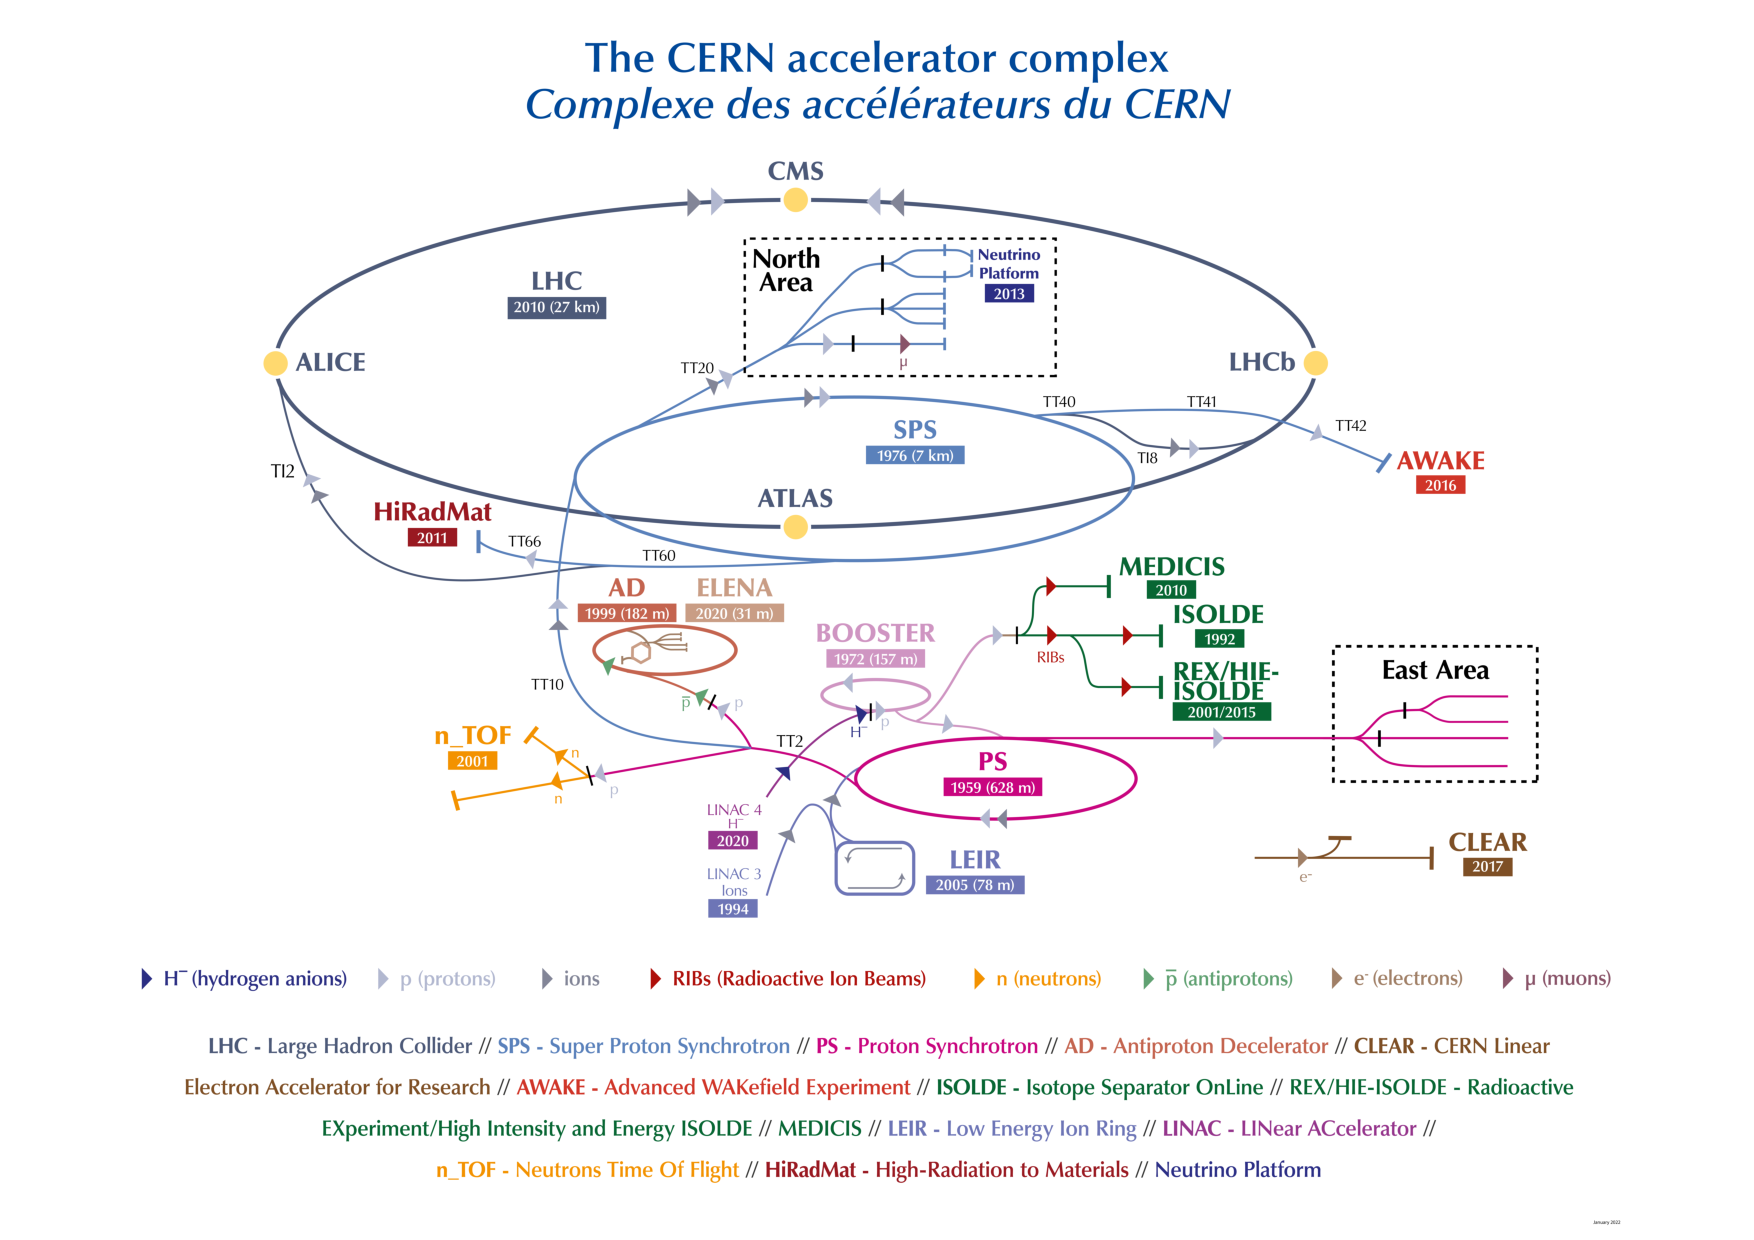
\includegraphics[width=0.5\linewidth]{figures/CCC-v2022.pdf}
    \caption{The CERN accelerator complex in 2022.\cite{Lopienska:2800984}}
    \label{fig:cern-acc-comp}
\end{figure}

\section{The ATLAS Experiment} \label{sec:atlas}

\section{Particle Reconstruction} \label{sec:reco}

\section{Dedicated Reconstruction for LLP Searches} \label{sec:llp_reco}

\chapter{Analysis Overview}
\label{chap:ana_overview}
The LHC provides a unique opportunity to search for weakly coupled $\mathcal{O}$(GeV) Heavy Neutral Leptons with the ATLAS detector given the large dataset of $W$-bosons. In 2022, the ATLAS experiment performed a search for HNLs, in the same final state targeted in this analysis, with the full Run-2 dataset~\cite{PhysRevLett.131.061803} (referred to as the 2022 analysis throughout this dissertation). However, the ATLAS object reconstruction algorithms have gone through significant improvement~\cite{atlascollaboration2023software} since then, opening up the opportunity to reanalyze the dataset with enhanced techniques and a better overall performance.~\Cref{sec:ana_goals} highlights the improvements in the reconstruction chain that the analysis benefits from and the corresponding new parameter space that these improvements unlock.~\Cref{sec:data_mc_samples} lists out the dataset and the Monte Carlo samples used in this search. Finally,~\cref{sec:object_sel} discusses the requirements imposed on the various objects used in this analysis.


\section{Analysis Goals}\label{sec:ana_goals}

This analysis searches for Heavy Neutral Leptons using 140.1 $fb^{-1}$ of $pp$ collision data recorded at $\sqrt{s}=13$~TeV in the $W\rightarrow \ela \mathcal{N}\left(\rightarrow\elb\elg\nu \right)$ final state. The charged lepton coming from the $W$ decay (\ela) is called the \textit{prompt} lepton since it appears to come from the primary $pp$ collision. Since the HNL is long-lived, the $\elb\elg$ system manifests as a two-pronged Secondary Vertex (SV) or Displaced Vertex (DV)\footnote{secondary, because the $pp$ collision and the $W$ production and decay gives the primary vertex, and displaced, because the the HNL has a proper lifetime long enough to resolve the PV and the SV.}, and \elb~and \elg~are called \textit{displaced} leptons. The ATLAS ID has the highest granularity (in the $\eta-\phi$ directions) out of all the sub-detector systems, making it the most adept at reconstructing the position and the kinematics of this DV. Hence, the analysis targets a reconstructed two-track DV in the ID volume. The reconstruction selection criteria, or cuts, on the ID tracks (specifically the $|d_0|\leq 300$~mm cut and the minimum number of hits) automatically impose a requirement that the DV radial position ($r_\mathrm{DV}$) has to be within the first layer of the strips silicon detectors (see~\cref{fig:inner-det}). Furthermore, the SV is required to be displaced ($r_\mathrm{DV}>4$~mm), adding a minimum requirement on the radial distance between PV and the DV in the radial direction. Finally, \ela, \elb, \elg~are required to be either $\mu$ or $e$, since $\tau$-leptons are unstable and decay rapidly. The electric charge of \ela~follows that of the $W$ boson, while \elb~and \elg~are oppositely charged. The goal of this analysis can hence be summarized as:

\textbf{A search for Heavy Neutral Leptons in decays of $W$ bosons in events with a prompt muon or electron, and a two-track displaced vertex in the Inner Detector volume of ATLAS with outgoing oppositely charged muons or electrons.}

\subsection{Reconstruction improvements}
The final state probed in this analysis is non-standard, since the primary ATLAS reconstruction chain is designed around reconstructing signatures from prompt particle decays, as described in~\cref{sec:reco}. Dedicated reconstruction techniques, such as LRT, add significant sensitivity to this final state. The 2022 analysis used an older, computationally expensive version of LRT which was only run on about 10$\%$ of the events retained by the ATLAS triggers based on a pre-defined set of filters. Furthermore, the LRT pass used for the 2022 analysis reconstructed a significant amount of ``fake" tracks, which inflated the amount of background faced. Lastly, LRT was only run for HNL signal Monte Carlo samples and not for other SM samples, which inhibited the usage of Monte Carlo-driven background estimation techniques. 

The analysis presented in this dissertation overcomes all of these challenges thanks to the vast improvement in reconstruction techniques, specifically in LRT. The new optimized LRT deployed for reconstruction in Run-3~\cite{IDTR-2021-03} was retroactively applied to data collected in Run-2 and all Monte Carlo simulations prepared for Run-2 conditions. The computational costs are significantly lowered, removing the need for filtering of events, making it possible to look for LLP events in all ATLAS data. The optimization significantly reduces the rate of fake tracks (and hence non-LLP SVs) reconstructed by the LRT chain while maintaining high signal efficiency as illustrated in~\cref{fig:LRT-fakeRate}, which compares the number of reconstructed DVs (both, genuine LLP and fake, i.e. non-LLP) between the legacy (implementation used in the 2022 analysis) and updated LRT reconstruction as a function of $r_\mathrm{DV-PV}$ (or $L_\mathrm{xy}$) using as a benchmark a simulated sample of $H\rightarrow aa \rightarrow b\bar{b}b\bar{b}$, where $a$ is an LLP.

\begin{figure}[!ht]
    \centering
    \includegraphics[width=0.6\linewidth]{figures//analysis_overview/LRT_fakeRate.pdf}
    \caption{A comparison of the radial distributions of reconstructed secondary vertices in a simulated LLP sample using the legacy and updated track reconstruction configurations.~\cite{IDTR-2021-03}}
    \label{fig:LRT-fakeRate}
\end{figure}


\subsection{Target Phase Space}

The vast improvements in LRT warrant a new search for displaced HNLs in leptonic final states using the full Run-2 dataset.~\Cref{fig:HNL-summ-mu} summarizes the current limits imposed on the square of the coupling of the HNL to a muon neutrino ($|U_{\mu\mathcal{N}}|^2$) in a single-flavor mixing scenario. The 2022 ATLAS analysis, shown in grey, excluded HNLs in the 1-10 GeV mass range with the corresponding lower limits on $|U_{\mu\mathcal{N}}|^2$ lying in the 10$^{-4}$ and 2$\cdot$10$^{-7}$ order. The analysis described in this thesis aims to expand the 2022 exclusion contour in all directions. Specifically, expansion to lower couplings in the 1-3 GeV \mhnl range probes HNL parameter spaces untouched by any other experiment. Furthermore, expanding to exclude \mhnl$>$10 GeV with couplings smaller than 10$^{-6}$ allows the exploration of completely new parameters. The former goal is achievable by more advanced background estimation methods, since the $\mathcal{O}$(GeV) \mhnl regions are generally dominated by background from hadronic decays. The latter goal is achievable by exploiting the improved LRT and DV reconstruction, since that phase space is limited by background with DVs from uncorrelated track crossings.

\begin{figure}[!ht]
    \centering
    \includegraphics[width=1\linewidth]{figures/analysis_overview/HNL_summary_mu.png}
    \caption{Summary of exclusion limits imposed by various experiments on the square of the coupling of Heavy Neutral Leptons to the muon neutrino as a function of the HNL mass. The limits imposed by the ATLAS 2022 analysis is shown in grey as ATLAS (2022).~\cite{Fernandez-Martinez:2023phj}}
    \label{fig:HNL-summ-mu}
\end{figure}

\section{Dataset and Monte Carlo Simulations}\label{sec:data_mc_samples}
\subsection{ATLAS dataset}
The full Run-2 ATLAS dataset used for this analysis corresponds to an integrated luminosity of 140.1 $fb^{-1}$ of $pp$ collisions at $\sqrt{s}=$13~TeV. Only the subset of events (satisfying the Good Run Lists) are considered which have passed detector condition and data quality thresholds to ensure the data are suitable for physics analysis. The amount of data collected is roughly correlated to the pileup during a set period, since the collision rate is larger when a higher number of protons are squeezed together in a bunch.

The ATLAS data goes through a reconstruction chain as described in~\cref{sec:reco}, and is stored in a data format called Analysis Object Data (AOD). These files, due to the presence of low-level event information, are large in size and are designed to be used across ATLAS analyses. A further skimming is applied on these files based on specific analysis needs.
Given the non-standard nature of physics objects and reconstruction methods used in this analysis, a specialized data format, called DAOD\_LLP1, is used. This Derived AOD (DAOD) format adds information for a large breadth of analyses searching for LLPs which wouldn't be available in the standard DAOD formats. The secondary vertexing algorithm used in this analyses requires low-level track information which are available in the AODs but not in the DAODs, and hence is run at the AOD$\rightarrow$DAOD\_LLP1 step. 

\subsection{Simulated Samples}
The signal and background processes affecting this analysis are simulated using Monte Carlo (MC) event generation. These simulations start with the event generation of the underlying hard-scatter event along with the parton shower process. The simulation is followed by the modeling of the interaction of the particles with the active detector material done using the \textsc{Geant4}~\cite{AGOSTINELLI2003250} simulation toolkit. In the next step, additional $pp$ interactions are overlaid along with the hard-scatter according to the data taking conditions of a corresponding year, and the whole event goes through a digitization step where the detector readout response is simulated to represent the signature left by real particles in ATLAS. Three MC campaigns are simulated - mc20a, d, and e, corresponding to the pileup and detector conditions in the years 2015-16, 2017, and 2018, respectively. The simulated pileup profile is reweighted to match the total integrated luminosity of the data taking period. The digitized signature is reconstructed to build physics objects in the AOD format. Finally, DAOD\_LLP1 are created for both data and MC samples to ensure the same treatment is applied to both.

\subsection*{Signal MC Samples}
Signal samples were generated using \textsc{MadGraph5\_aMC@NLO}~\cite{Alwall:2014hca} with HeavyN UFO model libraries~\cite{PhysRevD.94.053002} that provide a minimal SM extension with HNLs at next-to-leading order QCD accuracy and uses the \textsc{NNPDF3.0nlo}~\cite{Ball:2014uwa} set of PDFs. The events were interfaced to \textsc{Pythia\,8.230}~\cite{Sjostrand:2014zea} to model the parton shower, hadronization, and underlying-event, with parameters set according to the A14 tune~\cite{ATL-PHYS-PUB-2014-021} and using the \textsc{NNPDF2.3nlo}~\cite{Ball:2012cx} PDFs.

The $W$ boson from the primary $pp$ interaction is required to decay into a muon or an electron, and an HNL admixture ($W\to\ell\mathcal{N}$). The HNL is given a long lifetime and set to decay leptonically ($\mathcal{N}\to\ell\ell\nu$, $\ell=\mu$ or $e$, $\nu$ is the SM neutrino). The decay is modeled via a V-A weak matrix element, and can be mediated either via a virtual $W^*$ or $Z^*$. Both diagrams contribute to the decay if the charged leptons in the HNL decay have the same flavor. Samples are created with mean decay lengths \ctau~= 1, 10, 100 mm and masses \mn~= 1, 2, 3, 4, 5, 7.5, 10, 12.5, 15, 17.5, 20 GeV. For masses up to 5 GeV, \ctau~= 1000 mm is also considered. Both lepton-number conserving and violating decays are simulated.

The various models considered in this analysis are summarized in~\cref{tab:hnl_models}. The simulated samples are scaled to different cross-sections based on the final state and the model being considered. Six decay modes are considered in this analysis determined by the flavor of the charged leptons. The channels are represented as $\ell_\alpha - \ell_\beta \ell_\gamma$, where $\alpha$ is the flavor of the prompt lepton, and $\beta$ and $\gamma$ are the flavors of the charged leptons from the HNL decay.~\Cref{tab:channels} summarizes the six final states considered in this analysis and the decay modes that lead to that final state. $\ell_\beta$ and $\ell_\gamma$ cannot be experimentally resolved and neutrinos flavors cannot be observed using the ATLAS detector. Hence, the $\ell_\beta\ell_\gamma\nu$ and $\ell_\gamma\ell_\beta\nu$ contributions are combined.


\begin{table}[!ht]
    \centering
    \begin{tabular}{ccc}
        \hline\hline
         Final state/\ & \multicolumn{2}{c}{Decay mode from model with} \\
         Channel & Single flavor mixing HNL &  $\mu-$ and $e-$ mixing HNL \\
         \hline
         \uuu & $W\to\mu\mathcal{N}\left(\to\mu\mu\nu_\mu\right)$  & $W\to\mu\mathcal{N}\left(\to\mu\mu\nu_\mu + \mu\mu\nu_e \right)$\\
         \uue & $W\to\mu\mathcal{N}\left(\to\mu e\nu_e\right)$ & $W\to\mu\mathcal{N}\left(\to\mu e\nu_e + e\mu\nu_\mu \right)$\\
         \uee & $W\to\mu\mathcal{N}\left(\to e e\nu_\mu\right)$ & $W\to\mu\mathcal{N}\left(\to e e\nu_\mu + e e\nu_e\right)$\\
         \eee & $W\to e\mathcal{N}\left(\to e e \nu_e\right)$ & $W\to e\mathcal{N}\left(\to e e \nu_e +  e e \nu_\mu\right)$\\
         \eeu & $W\to e\mathcal{N}\left(\to e \mu\nu_\mu\right)$ & $W\to e\mathcal{N}\left(\to e \mu\nu_\mu + \mu e\nu_e\right)$\\
         \euu & $W\to e\mathcal{N}\left(\to\mu\mu\nu_e\right)$ & $W\to e\mathcal{N}\left(\to\mu\mu\nu_e + \mu\mu\nu_\mu\right)$\\
         \hline\hline
    \end{tabular}
    \caption{The six final states considered in this analysis and the decay modes that contribute to them for the different mixing models considered.}
    \label{tab:channels}
\end{table}

\subsection*{Background MC Samples}
MC simulations are used to model the kinematics of the (correlated) background from SM processes contaminating the phase space explored in this analysis. Specifically, simulations of the top-quark pair production ($t\bar{t}$) and $V+$jets ($V=W,\xspace Z$) processes are considered.

The production of $t\bar{t}$ events was modelled using the \textsc{Powheg\,Box\,v2}~\cite{Frixione:2007nw,Nason:2004rx,Frixione:2007vw,Alioli:2010xd} generator at next-to-leading order with the \textsc{NNPDF3.0nlo}~\cite{Ball:2014uwa} PDF set and the \hdamp~parameter\footnote{The \hdamp~parameter is a resummation damping factor and one of the parameters that controls the matching of \textsc{Powheg} matrix elements to the parton shower and thus effectively regulates the high-\pT radiation against which the $t\bar{t}$ system recoils.} set to 1.5\,$m_{\mathrm{top}}$~\cite{ATL-PHYS-PUB-2016-020}.  The events were interfaced to \textsc{Pythia\,8.230}~\cite{Sjostrand:2014zea} to model the parton shower, hadronisation, and underlying event, with parameters set according to the A14 tune~\cite{ATL-PHYS-PUB-2014-021} and using the \textsc{NNPDF2.3lo} set of PDFs~\cite{Ball:2012cx}. The decays of bottom and charm hadrons were performed by \textsc{EvtGen\,1.6.0}~\cite{Lange:2001uf}. The non-all-hadronic slice of the sample is used, which includes leptonic final states.

The $W(\rightarrow \ell\nu)+$jets and $Z(\rightarrow \ell\ell)+$jets samples are generated using \textsc{Sherpa2.2.11}~\cite{Gleisberg:2008ta,Hoeche:2009rj,Bothmann:2019yzt} at next-to-leading order accuracy up to 2 jets, and up to leading order accuracy for up to 5 jets in the Matrix Element. The samples are created in three slices of the flavor of the jets, namely BFilter, CFilterBVeto, and CVetoBVeto, where XFilterYVeto refers to samples where a jet with flavor X is required and a jet with flavor Y is vetoed. Furthermore, for $\tau$ final states, the samples are divided by the decays of the $\tau$ lepton as either leptonic or (semi-)hadronic. For the predictions used in this analysis, all the slices and filters are combined for the total expected event yield.
 
\subsection{Signal Kinematics}
The position of the HNL decay depends on its proper lifetime and its boost, and the kinematics of its decay products depend on its mass and its boost.~\Cref{fig:truth_kinematics} shows some representative kinematic distributions of the HNL and its decay products at the \textit{truth level}, i.e. the actual kinematics of the simulated particles inside the ATLAS experiment. Such distributions are typically contrasted against kinematics at the \textit{reconstructed level}, i.e. kinematics after digitization, reconstruction, and identification of the same simulated particles.

\begin{figure}[!ht]
    \centering
     \subfloat[HNL decay radius]{\includegraphics[width=0.45\textwidth]{figures/analysis_overview/TruthKinematics/rProd.pdf}\label{fig:kinem_rprod}}
     \subfloat[$\mu$ or $e$ $|d_0|$ ]{\includegraphics[width=0.45\textwidth]{figures/analysis_overview/TruthKinematics/lepD0.pdf}\label{fig:kinem_d0}} \\
     \subfloat[$\mu$ or $e$ \pT]{\includegraphics[width=0.45\textwidth]{figures/analysis_overview/TruthKinematics/lepPt.pdf}\label{fig:kinem_pt}}
     \subfloat[$\mu$ or $e$ $\eta$]{\includegraphics[width=0.45\textwidth]{figures/analysis_overview/TruthKinematics/lepEta.pdf}\label{fig:kinem_eta}}
     \caption{Truth level kinematic distributions for \uue HNL samples for some representative masses and proper lifetimes indicated in the legend. The total entries for each histogram are normalized to 1 for a fair comparison comparison, and overflow (underflow) is shifted into the first (last) bin.}
     \label{fig:truth_kinematics}
 \end{figure}

In the frame of the HNL, the probability density for it to decay after a time $t$ is given by the exponential distribution:
\begin{equation}
    p_\mathrm{decay}(t)=e^{-t/\tau_\mathrm{HNL}}.
\end{equation}
In the lab frame, the radial position of the HNL decay, as illustrated in~\cref{fig:kinem_rprod}, depends on both its mass and proper lifetime due to a time dilation effect from its Lorentz boost. The track reconstruction efficiency drops after 300 mm due to the lack of enough silicon hits in the ID, causing most of the HNL decays for \ctau = 100 mm and 1000 mm to lie outside acceptance.~\Cref{fig:kinem_d0} shows the $|d_0|$ distribution for the charged decay products of the HNL which is independent of the mass of the HNL for a fixed proper lifetime. LRT adds sensitivity to higher lifetime HNLs since they have a large proportion of decays with $|d_0|>5\,$mm.~\Cref{fig:kinem_pt,fig:kinem_eta} show that the \pT and $\eta$ spectrum of the HNL decay products have a weak dependency on the mass and the lifetime being considered, especially in the \mhnl$<<m_W$ regime, where most of the momentum from the $W$ decay is transferred to the prompt lepton.

After studying the truth-level kinematics of the HNL signal, the simulated samples are used to quantify the detector acceptance and reconstruction efficiencies of the HNL samples as shown in~\cref{fig:acc_and_eff}.

\begin{figure}[!ht]
    \centering
     \subfloat[Acceptance Categorization]{\includegraphics[width=0.45\textwidth]{figures/analysis_overview/TruthKinematics/plots_truth_eff_stack.pdf}\label{fig:categ_truth}}
     \subfloat[Reconstruction Categorization]{\includegraphics[width=0.45\textwidth]{figures/analysis_overview/TruthKinematics/plots_reco_eff_stack.pdf}\label{fig:categ_reco}}
     \caption{Fractional detector acceptance, ID track reconstruction, and muon reconstruction efficiencies for \uuu HNL samples for some representative mass and proper lifetimes indicated on the $x-$axis.}
     \label{fig:acc_and_eff}
 \end{figure}

~\Cref{fig:categ_truth} classifies HNL di-muon decays according to the detector and kinematic acceptance (\pT$>3$~GeV, $|\eta|<2.7$) of a truth muon and if the truth muon leaves hits that are reconstructed as an ID track. The fraction of events where both muons are reconstructed as tracks is within 5-60\% with a strong dependence on the HNL proper lifetime and a weak dependence on its mass, since they affect the production radius of the muons and hence their tracking acceptance.~\Cref{fig:categ_reco} further categorizes the cases with two reconstructed ID tracks according to their muon extension efficiency i.e. if the ID tracks are matched to reconstructed muons. A stronger (yet still subtle in the masses considered) dependency is observed on the HNL mass than lifetime, since the \pT spectrum of the muons are skewed towards higher values for heavier HNLs, as shown in~\cref{fig:kinem_pt}. Hence, low mass and high lifetime HNLs suffer from low detector acceptance and low lepton reconstruction efficiencies. This fact, further convoluted with the low cross-section of HNL production in that phase space, makes the exploration of lighter and weakly-coupled HNLs extremely challenging.

\section{Physics Objects Selection}\label{sec:object_sel}
The final state probed in this analysis is characterized by a prompt lepton and a displaced vertex in the ID volume with two outgoing leptons. Furthermore, some requirements on the quark flavor of jets in the event are imposed in the definition of analysis regions.

\subsection{Prompt Lepton and Trigger}
A prompt lepton is defined as a muon or an electron coming from the primary $pp$ interaction. The prompt lepton is used as the primary triggering object to tag the $W$-decay, and hence, the requirements on the selection of the prompt lepton are driven by the selections imposed by the trigger chain. The identification Working Point (WP) adds self-consistency and goodness of fit requirements on the lepton object to select genuine leptons against incorrect combinations of hits or hadron decays-in-flight. Similarly, isolation separates leptons without hadronic or radiative activity around them, as is expected from $W\to\ell\nu$, from those that are within jets. Finally, track-to-vertex association requires that the lepton points back to the primary $pp$ collision.~\Cref{tab:plep_selection} summarizes the selections imposed on the prompt lepton candidate.

\begin{table}[!ht]
    \centering
    \resizebox{\columnwidth}{!}{
    \begin{tabular}{cc}
        \hline\hline
        Cut Name & Cut Description \\
        \hline
        Lepton Flavor & muon or electron \\
        Trigger Matched & $\checkmark$ \\
        Transverse Momentum & \pT $>$ 27 GeV \\
        Identification Working Point & \texttt{Medium}~\cite{MUON-2018-03,PERF-2017-01} \\
        Isolation Working Point & \texttt{PflowLoose\_VarRad}~\cite{MUON-2018-03} (\texttt{Loose\_VarRad}~\cite{EGAM-2018-01}) for $\mu\,(e)$ \\
        Track-to-Vertex-Association & $|d_{0}/\sigma(d_{0})| < 3\,(5)$ for $\mu\,(e)$, $|z_{0}\sin{\theta}| < 0.5$ mm~\cite{MUON-2018-03,EGAM-2018-01} \\
        \hline\hline
    \end{tabular}
    }
    \caption{Selections used for the prompt lepton candidate.}
    \label{tab:plep_selection}
\end{table}

If more than one prompt lepton candidate are found in an event, the candidate with the highest transverse momentum is chosen as the prompt lepton.

\begin{table}[!ht]
    \centering
    \begin{tabular}{ccc}
        \hline\hline
        Period & Muon Trigger & Electron Trigger \\
        \hline
        2015 & HLT\_mu20\_iloose\_L1MU15 & HLT\_e24\_lhmedium\_L1EM20VH \\
        2016, 2017, 2018 & HLT\_mu26\_ivarmedium & HLT\_e26\_lhtight\_nod0\_ivarloose \\
        \hline\hline
    \end{tabular}
    \caption{Lowest unprescaled single lepton triggers used in the analysis.}
    \label{tab:triggers}
\end{table}

The lowest unprescaled single lepton triggers are used in this analysis, with the exact trigger scheme for each data taking year listed in~\cref{tab:triggers}. ~\Cref{fig:trigger_eff} shows the fraction of events where a single lepton fires the trigger as a function of the prompt lepton \pT for the single muon and single electron triggers for a selection of \uuu and \eee signal samples. The low \pT tail on the plots come from events in which the lepton causing the trigger originated from the displaced leptons. This tail would disappear once the selections on the prompt lepton are applied. The selections in~\cref{fig:trigger_eff} are limited to the presence of a PV, a prompt lepton (without any selections), and the presence of a $\mu\mu$ or $ee$ DV in the fiducial volume.

\begin{figure}[!ht]
    \centering
     \subfloat[\uuu \mn=10 GeV]{\includegraphics[width=0.45\textwidth]{figures/analysis_overview/trigger/effbylifetime_uuu.pdf}}
     \subfloat[\eee \mn=10 GeV]{\includegraphics[width=0.45\textwidth]{figures/analysis_overview/trigger/effbylifetime_eee.pdf}} \\
     \subfloat[\uuu \ctau=10 mm]{\includegraphics[width=0.45\textwidth]{figures/analysis_overview/trigger/effbymass_uuu.pdf}}
     \subfloat[\eee \ctau=10 mm]{\includegraphics[width=0.45\textwidth]{figures/analysis_overview/trigger/effbymass_eee.pdf}}
     \caption{Fraction of events where any single-lepton trigger is fired by any lepton as a function of the prompt lepton \pT for a selection of HNL signal mass and lifetimes for the \uuu and \eee channels.}
     \label{fig:trigger_eff}
\end{figure}

\subsection{Displaced Muons}
Muons in the displaced vertex are referred to as displaced muons. Since these muons are produced from a decay away from the IP, they are not always expected to point back to it. Hence, to extend the analysis coverage to such non-pointing muons, a combination of standard and LRT muons are used.

As described in~\cref{sec:reco}, the standard (i.e. both primary and inside-out) muon reconstruction and LRT muon reconstruction run seperately using all the hits in the MS in an event as inputs along with the standard ID tracks for the former chain and the LRT tracks for the latter chain. This workflow, due to the use of all MS hits in both the chains, causes a large fraction of LRT muons to share MS hits (or rather a full MS track) with a standard muon. The LRT and standard muon are hence said to have an \textit{overlap} with each other. This is an unphysical situation since it's not possible for two genuine muons to leave identical MS hits. However, the muon reconstruction algorithm is very liberal in the quality of muons it reconstructs, and hence a bad quality LRT muon could overlap with a good quality standard muon, and vice versa. An overlap resolution strategy is designed to retain or reject a muon object from a pair (out of which one is reconstructed as a standard muon and the other as a LRT muon) which share an MS track between them. The strategy is optimized for maximal signal retention post overlap removal, and uses fundamental muon quality requirements without adding any biases from the kinematics of the signal. In case both or neither muon passes a check, the resolution moves on to the next check. The overlap resolution is designed to, in case of a MS track overlap, retain the muon which passes these requirements, followed sequentially:
\begin{itemize}
    \item passes the \texttt{Loose}~\cite{MUON-2018-03}\footnote{The \texttt{Loose} criteria used here is modified to not apply any requirements on the ID track.} identification working point,
    \item is a Combined muon,
    \item has a lower absolute $\eta$ difference between the measurement from ID track and the MS track extrapolated to the perigee,
    \item is reconstructed in the standard pass (fallback option).
\end{itemize}
~\Cref{fig:muon_overlap} shows the fraction of standard and LRT muons which have an overlap at different stages of the overlap removal process.

\begin{figure}[!ht]
    \centering
    \includegraphics[width=0.75\linewidth]{figures//analysis_overview/plots_muon_overlap_fraction_AllStages.pdf}
    \caption{Fraction of standard and LRT muons that have MS track overlaps at different stages of the overlap removal process.}
    \label{fig:muon_overlap}
\end{figure}

After the standard and LRT muon collections are combined and the overlaps are resolved, they are treated similarly for downstream analysis. Only Combined displaced muons are used in this analysis with the kinematic requirements of \pT$>3$~GeV and $|\eta|<2.5$, both of which are imposed by muon reconstruction and detector constraints. A \texttt{Medium} identification WP is used to identify genuine muons against pion decays. However, the application of the WP is modified for LRT muons. LRT reconstruction has, by design, stringent reconstruction criteria as shown in~\cref{tab:std-lrt-diff}. Hence, the \texttt{Medium} ID WP for LRT muons is slightly modified to not apply the above requirements on the ID tracks while retaining the other cuts.~\Cref{tab:disp_muon_selection} lists the cuts imposed on the identification of displaced muons.

\begin{table}[!ht]
    \centering
    \begin{tabular}{cc}
        \hline\hline
        Cut Name & Cut Description \\
        \hline
        Transverse Momentum & \pT $>$ 3 GeV \\
        Pseudo-rapidity & $|\eta|<2.5$ \\
        Muon Type & Combined \\
        Identification Working Point & \texttt{Medium} (w/o ID cuts for LRT muons) \\
        \hline\hline
    \end{tabular}
    \caption{Selection criteria used for displaced muons.}
    \label{tab:disp_muon_selection}
\end{table}


\subsection{Displaced Electrons}
Electrons in the displaced vertex are referred to as displaced electrons. Similar to muons, a combination of standard and LRT electrons are used to identify displaced electrons. The standard and LRT electron reconstruction use the same calorimeter information for each event, and hence, a standard electron and an LRT electron can point to to the same calo-cluster. These \textit{overlaps} are resolved by using the trigger-level identification WPs as defined in~\cite{PERF-2017-01}. Out of an overlapping standard-LRT electron pair, the electron which passes a stricter\footnote{The \texttt{Tight} identification WP has the strictest requirements, followed by \texttt{Medium}, \texttt{Loose}, and \texttt{VeryLoose}.} identification WP requirement is retained. In the case where both the standard and LRT electron pass the same identification WP, the electron reconstructed from the standard pass is kept. The identification WPs used here are further loosened with respect to the trigger-level working points by relaxing the hard requirements on the number of silicon hits in the pixel sub-detectors. 

A \pT threshold of 4.5 GeV is imposed on displaced electrons driven by reconstruction requirements. No cuts beyond those imposed by detector limitations are applied on electron $\eta$. The \texttt{VeryLooseNoPix} identification WP is used for the displaced electrons, which is the same as the \texttt{VeryLooseNoPix} trigger-level identification WP as defined in~\cite{PERF-2017-01} (which already uses a relaxed version of the WPs used for offline electron identification), but with the requirement on the number of silicon pixel hits removed to reduce the bias towards electrons emerging from the IP and add efficiency to electrons from LLP decays. The same identification WP is applied to both standard and LRT electrons. Since the WP imposes very relaxed requirements on the electron, an extra requirement on the compatibility of the \pT of the electron object and its corresponding GSF track is imposed to reject mismatches that would arise from photon radiation. Such a cut ensures that the final state identification, which is based on the electron object, and the DV kinematics reconstruction, which is based on the track object, are compatible to each other.~\Cref{tab:disp_electron_selection} lists the cuts imposed on the identification of displaced electrons.

\begin{table}[!ht]
    \centering
    \begin{tabular}{cc}
        \hline\hline
        Cut Name & Cut Description \\
        \hline
        Transverse Momentum & \pT $>$ 4.5 GeV \\
        Identification Working Point & \texttt{VeryLooseNoPix}\\
        Momentum Balance & $|\pT^\mathrm{electron}-\pT^\text{GSF track}|/\pT^\mathrm{electron}<0.5$ \\
        \hline\hline
    \end{tabular}
    \caption{Selection criteria used for displaced electrons.}
    \label{tab:disp_electron_selection}
\end{table}

\subsection{b-tagged Jets}
At tree level, the HNL signal process in the fully leptonic final states has no hadronic activity. The leading source of jets in signal events is Initial State Radiation from the incoming partons which then showers to give jets. The chance of hence observing a jet (which have a reconstruction \pT threshold of 20 GeV) is low, and a jet from a b-quark is even lower. This fact is used to define analysis regions rich in background and highly depleted in the signal process.

This analysis uses anti-$k_t$ $\Delta R =0.4$ PFlow jets reconstructed with \pT$>20$~GeV and $|\eta|<4.9$ limited by the calorimeter coverage. Machine learning algorithms are trained to learn about the substructure of jets to classify jets initiated by heavy ($b$ or $c$) quarks against those initiated by light quarks or gluons. In this analysis, the DL1d tagger~\cite{ATL-PHYS-PUB-2022-047} is used to identify the flavor of jets. DL1d is based on a deep neural network. It takes information about the secondary vertex reconstructed inside jets and other low level information about jet substructure and returns a classification score. A cut on the DL1d tagger score of a jet which accepts on average 85\% of jets with b-hadrons, or the 85\% b-jet efficiency WP, is applied to identify jets as either coming from b-quarks, or lighter quark flavors. A jet passing the 85\% WP cut of the DL1d tagger score is called a b-tagged jet or a b-jet.

\subsection{Overlap Removal}
This analysis makes use of reconstructed electron, muon, and jet physics objects. Since the reconstruction chains of these objects run in parallel, it is possible that such objects share ID tracks or calo-clusters. An overlap removal (where the overlap criteria based on the type of objects in context) step is run after the baseline selection of the physics objects but before using them for analysis. An overlap removal strategy which favors leptons over jets is used in this analysis. This choice was shown to have a negligible impact on the signal significance in the measured phase space as compared to the standard ATLAS overlap removal strategy. However, a significant increase in the event yield was seen in a non-overlapping analysis region which is used to constrain correlated background contribution. The non-overlapping region is used to collect events with leptons inside jets the statistics of which are increased by using this overlap removal strategy, which led to a better data-driven estimate of the background yield.~\Cref{tab:overlap_removal} lists the rules used for resolving overlaps between physics objects according to the criteria of overlap between them, run sequentially from top to bottom.

\begin{table}[!ht]
    \centering
    \begin{tabular}{ccc}
        \hline\hline
        Reject & Against & Overlap Criteria \\
        \hline
        electron$^1$ & electron$^2$ & shared ID track, $\pT^1 < \pT^2$ \\
        muon & electron & is CT-muon and shared ID track \\
        electron & muon & shared ID track \\
        jet & electron & $\Delta R<0.2$ \\
        jet & muon & \#tracks in jet $<$3 and (ghost-associated\footnotemark or $\Delta R<0.2$) \\
        \hline\hline
    \end{tabular}
    \caption{The lepton-favored overlap removal scheme and overlap criteria.}
    \label{tab:overlap_removal}
\end{table}
\footnotetext{Particles are assigned to jets following the ghost-association procedure which consists of assigning them to jets by adding their tracks with infinitesimal \pT to the jet clustering process. A particle is hence ghost-associated to a jet if it is retained after the jet clustering.}

\subsection{Secondary Vertex Reconstruction and Selection}
The track selection, DV reconstruction, and DV selection is facilitated by a package called Vertex Secondary Inclusive (VSI)~\cite{ATL-PHYS-PUB-2019-013} at the core of which is the vertex reconstruction algorithm, VkalVrt~\cite{Kostyukhin:685551}.

\begin{figure}[!ht]
    \centering
    \includegraphics[width=0.8\linewidth]{figures//analysis_overview/vertexing/VSIalg.png}
    \caption{The main steps used for secondary vertex reconstruction in the Vertex Secondary Inclusive algorithm.~\cite{ATL-PHYS-PUB-2019-013}}
    \label{fig:vsi-steps}
\end{figure}

~\Cref{fig:vsi-steps} summarizes the steps followed by VSI for DV reconstruction. The first step of the algorithm is the selection of tracks used to seed the reconstruction. A large number of tracks arise from pileup in the current LHC conditions which are not of physics interest for searches such as ours. Hence, a strict selection of tracks is important to reduce the combinatorics and hence chances of reconstructing a DV which comes from a fake crossing rather than a genuine decay. These pre-selected tracks are used to create pairs in a two-track seed finding which checks their compatibility as DV track candidates, followed by a $\chi^2$ minimizing fit. Since a track can be attached to multiple seeded pairs, such cases are resolved in the next step by checking for incompatibilities of a track in an n-track vertex, based on a goodness of fit score. Multiple secondary vertices corresponding to a single LLP decay can be reconstructed by this algorithm. To combine these candidates, DVs with low track multiplicity are attempted to be refit with DVs with higher track multiplicities requiring the refitted DV position and the original DV position to be compatible. In the final step, tracks that are not part of any DVs are attempted to be attached to the reconstructed DVs if they increase the goodness of fit score.

This analysis uses the same steps and configurations as outlined in~\cite{ATL-PHYS-PUB-2019-013}, apart from a few but significant notable differences which result in improved signal acceptance and significant reduction in uncorrelated background:
\begin{itemize}
    \item Since the final state probed in this analysis is fully leptonic, the track pool used for seeding is modified to use
    \begin{enumerate}
        \item ID tracks matched to CB or ST muons,
        \item GSF tracks matched to electrons, and
        \item other non-leptonic ID tracks
    \end{enumerate}
    in each event. GSF tracks have better $d_0$ and $z_0$ resolution than standard ID tracks for electrons and hence result in better reconstruction efficiency for DVs with electrons. Other non-leptonic ID tracks are added to all events to expand sensitivity to lepton+track like final states which would result from semi-leptonic decays of the HNL which are planned to be studied in the near future. 
    \item At the two-track vertex finding level, the minimum $|d_0|$ requirement on the pair of tracks is reduced from 2 mm (as is in the standard algorithm) to 1 mm. An error was found in the technical implementation of this cut which led to the accidental acceptance of a significant number of DVs failing this requirement in the 2022 analysis. This error was fixed for this version of the analysis, leading to a significant reduction in correlated background and a near elimination of uncorrelated background.
    \item The track attachment is modified to only use tracks from the seeding pool. This reduces the unwanted promotion of genuine two-track signal vertices to three-track vertices with one accidental track crossing, say from pileup. Such a change increases signal acceptance since, in the analysis, $n$-track vertices are vetoed, where $n>2$.
    \item As a last stage cleaning, all DVs without any tracks matched to leptons are removed.
\end{itemize}

The reconstruction efficiency of DVs is defined as the rate of having a reconstructed vertex matched to an individual HNL decay. To study the tracking and vertexing performance separately from each other, the total efficiency is factorized into independent terms. The efficiencies are defined as follows:
\begin{itemize}
    \item \textbf{Acceptance, $\mathcal{A}$}: fraction of all HNL decays with two charged particles with \pT $>1$~GeV, a true LLP decay $z$ position of $|z|<2720$~mm (inner surface of the last endcap layer), and a transverse distance from the origin of $r_\mathrm{DV}<563$~mm (inner surface of the TRT). The first requirement ensures that the vertex has decay products have large enough momentum to be reconstructed by the tracking algorithm, while the latter two ensure that the HNL was produced within the tracking volume of the ID. The definition of acceptance is purely based on the geometry of the ID without taking into account the limits of track reconstruction, which become more relevant in the next term, the seed efficiency.
    \item \textbf{Seed efficiency, $\varepsilon_\mathrm{seed}$}: fraction of accepted HNL decays having two reconstructed tracks passing the ID track selection requirements. The seed efficiency determines the performance of the object reconstruction algorithms convoluted with the effect of the track seeding cuts.
    \item \textbf{Core efficiency, $\varepsilon_\mathrm{core}$}: fraction of seeded HNL decays having a matched reconstructed vertex.
    The matching of ID tracks to truth particles is based on a weighted scoring of shared detector hits between the track and truth particle trajectories. For each pair of a reconstructed vertex $v$ and a truth HNL decay vertex $l$, a truth-matching score $s$ is computed using the magntitude of the track \pT as a weight. The score is given by:
    \begin{equation}
        s(v, l) \equiv \frac{\sum_{i \in \text { tracks } \in v}\left(\pT^{(i)} \mid \text { descendent of HNL decay } l\right)}{\sum_{i \in \text { tracks } \in v} \pT^{(i)}}
    \end{equation}
    A reconstructed vertex $v$ is said to match to a truth vertex $l$ if the score $s(v,l)>0.5$. The core efficiency represents the true performance of the vertexing algorithm itself with the track acceptance and reconstruction effects factored out.
\end{itemize}

The \textbf{total efficiency ($\varepsilon_\mathrm{total}$)}, is given by
\begin{equation}
    \varepsilon_\mathrm{tot}=\mathcal{A}\cdot\varepsilon_\mathrm{seed}\cdot\varepsilon_\mathrm{core}.
\end{equation}

\begin{figure}[!ht]
    \centering
     \subfloat[Acceptance]{\includegraphics[width=0.45\textwidth]{figures/analysis_overview/vertexing/LC_acc.pdf}}
     \subfloat[Seed efficiency]{\includegraphics[width=0.45\textwidth]{figures/analysis_overview/vertexing/LC_seed.pdf}} \\
     \subfloat[Core efficiency]{\includegraphics[width=0.45\textwidth]{figures/analysis_overview/vertexing/LC_core.pdf}}
     \subfloat[total efficiency]{\includegraphics[width=0.45\textwidth]{figures/analysis_overview/vertexing/LC_total.pdf}}
     \caption{The four efficiencies with the custom vertexing configuration as a function of $r_\text{DV}$ evaluated for the \uuu, \uue, and \uee channels with $\mn=2$ GeV, $\ctau=10$ mm.}
     \label{fig:VSILepTrack_sig_eff_LC}
\end{figure}

~\Cref{fig:VSILepTrack_sig_eff_LC} shows the four efficiencies as a function of $r_\text{DV}$, the radial distance of the HNL decay from its origin for a \mn=10 GeV, \ctau=10 mm benchmark HNL signal sample for the three DV flavor combinations $\mu\mu$, $e\mu$, and $ee$ under 2018 pileup and detector conditions. The flavor of the prompt lepton is irrelevant for this study. $\mathcal{A}$ is measured to be uniformly high at $\sim$80\% for all three flavors and falls off at high $r_\text{DV}$ values as the HNL starts to decay outside the ID acceptance. $\varepsilon_\mathrm{seed}$ is highest for $\mu\mu$ followed by $e\mu$ and $ee$. The \pT threshold for electron reconstruction is higher than that for muons (4.5 GeV as compared to 3 GeV), making $\varepsilon_\mathrm{seed}$ lower for LLPs decaying to electrons. Furthermore, a failure in reconstructing any of the two charged particles from the HNL decay would lead to a non-seeded vertex. This, along with the stringent requirements imposed by VSI on track quality, results in relatively low $\varepsilon_\mathrm{seed}$ across DV flavors and the full $r_\text{DV}$ range, with a sharp drop to 0 at $r_\text{DV}>300$~mm due to a drop in track reconstruction efficiency. $\varepsilon_\mathrm{core}$ is similar for all DV flavors. The losses at low $r_\text{DV}$ are driven by the cut on minimum track $|d_0|$. Furthermore, $\varepsilon_\mathrm{core}$ starts dropping at high $r_\text{DV}$ since, for a given mean proper lifetime, the average HNL boost increases with decay radius, resulting in more collimated decay products and a vertex topology which is more challenging to reconstruct. $\varepsilon_\mathrm{total}$ is hence seen to cap at 15-35\% for \mn=10 GeV, \ctau=10 mm HNL decays driven by the DV flavor.

Apart from the effects mentioned above, the DV reconstruction performance also depends on the pileup since a higher incidence of pileup tracks makes it difficult to separate genuine decays from decays from accidental track crossings.~\Cref{fig:vsi-pileup} shows $\varepsilon_\mathrm{total}$ for HNL decays in the \uuu channel for the three different MC campaigns, that correspond to the detector and pileup conditions of different data taking years and have pileup profiles as shown in~\cref{fig:pileup}. The signal DV reconstruction efficiency is observed to be robust against pileup differences whereas the effect is expected to be bigger on background since LRT fake rate increases with pileup.

\begin{figure}[!ht]
    \centering
    \includegraphics[width=0.5\linewidth]{figures/analysis_overview/vertexing/pileup_eff_total.pdf}
    \caption{Total vertex reconstruction efficiency of $\mn=2$ GeV, $\ctau=10$ mm HNL decays in the \uuu channel for the mc20a, mc20d, and mc20e campaigns.}
    \label{fig:vsi-pileup}
\end{figure}

DVs with exactly two outgoing tracks are considered, where both tracks are required to be either muons or electrons, with the displaced lepton quality requirements imposed on them. The number of events with more than one such DV are found to be negligible, hence the first DV passing these conditions is selected as the HNL candidate. \pT cuts are applied on the DV tracks to reject soft QCD background. Finally, a fiducial selection is applied to the radial position of the DV to ensure the decay happens inside the innermost strip layer of the ID and that the decay has a minimum level of displacement from the PV.~\Cref{tab:dv_selection} summarizes the cuts applied for selection of the DV candidate.

\begin{table}[!ht]
    \centering
    \begin{tabular}{ccc}
        \hline\hline
        Cut Name & Cut Description \\
        \hline
        Track multiplicity & exactly 2 \\
        Flavor & $\mu\mu,\,e\mu,\text{or }ee$ \\
        Track \pT & $\pT^\mathrm{lead}>10$~GeV, $\pT^\mathrm{sub-lead}>5$~GeV \\
        %Overlap Removal & $\Delta R(\text{DV tracks}, \text{prompt lep})>0.05$ \\
        Fiducial Cut & 4 mm $<\,r_\mathrm{DV}\,<$~300 mm\\
        \hline\hline
    \end{tabular}
    \caption{Selection criteria used for the displaced vertex.}
    \label{tab:dv_selection}
\end{table}


\chapter{Analysis Strategy}
\label{chap:ana_strategy}
The goal of this analysis is to search for long-lived Heavy Neutral Leptons in the 1-20 GeV mass range. While the displaced vertex driven search provides a clean signature to work with, there are various sources of backgrounds that contaminate the targeted phase space.~\Cref{sec:backgrounds} describes these backgrounds and the kinematic cuts that remove or reduce them.~\Cref{sec:corr_bkg} details the study of the background consisting of DVs with correlated tracks and its method of estimation.~\Cref{sec:uncorr_bkg} outlines the same for DVs with uncorrelated tracks. After all the background estimation methods are in place, the signal strength is extracted using a simultaneous fit across all analysis regions as described in~\cref{sec:sig_ext}.

\section{Backgrounds}\label{sec:backgrounds}
The backgrounds considered in this analysis are categorized into reducible and irreducible. While dedicated cuts are used to completely remove reducible backgrounds with negligible impact to the signal, cuts applied to suppress irreducible backgrounds also affect the signal, with the exact cut value optimized to maximize signal significance.

\subsection{Reducible backgrounds}
\begin{figure}[!ht]
    \centering
     \subfloat[$\gamma\to ee$ conversions]{\includegraphics[width=0.3\textwidth]{figures/analysis_strategy/bkg_illustrations/photon_conv.png}}
     \subfloat[Cosmic muons]{\includegraphics[width=0.3\textwidth]{figures/analysis_strategy/bkg_illustrations/cosmics.png}}
     \subfloat[$Z\to\ell\ell$ decays]{\includegraphics[width=0.3\textwidth]{figures/analysis_strategy/bkg_illustrations/zdecays_1.png}}
     \caption{Illustrative topology of the reducible backgrounds in the ATLAS ID volume.}
     \label{fig:bkg_reducible}
\end{figure}

Three sources of reducible backgrounds affect this analysis, as illustrated in~\cref{fig:bkg_reducible}:
\begin{enumerate}
    \item $\gamma\to ee$ conversions: Photons interacting with the various layers of material in the ID volume recoil against the atoms and produce a $e^+e^-$ pair. Such a $ee$ DV, along with a prompt lepton source, contaminates the measurement phase space. To remove this background, $ee$ DVs are required to be inside a narrower fiducial volume ($|z|<300$~mm) and must satisfy a \textit{material} veto, which rejects DVs which have a reconstructed position consistent with the position of the detector material. The material map, as shown in~\cref{fig:material_map}, is constructed using the known positions of detector elements and from the position of low-mass vertices reconstructed in data~\cite{SUSY-2018-13}. The material veto removes 48\% of the fiducial volume. The two electrons from a photon conversion are highly collinear since the recoiling nucleus takes very little momentum away from the photon. Hence, the \mdv distribution\footnote{$\mdv\approx\sqrt{E_1\cdot E_2 (1-\cos\alpha)+2m_1m_2}$ for relativistic objects with energies and masses $E_1,\,E_2$ and $m_1,\,m_2$, respectively.} starts at $\sqrt{2}m_e$ and falls sharply. Since the \mdv calculation makes a pion mass assumption on the outgoing tracks, the lower mass bound is given by $\sqrt{2}m_{\pi^+}\approx280$~MeV. Hence, to further reject any remaining conversions, a $\mdv>500$~MeV cut is applied on $ee$ DVs. This assumption does not affect the impact of the cut since an \mdv measurement of the scale $\sqrt{2}m_e$ cannot be resolved by ATLAS.

    \begin{figure}[!ht]
        \centering
        \subfloat[Positions in $x-y$ plane]{\includegraphics[width=0.5\textwidth]{figures/analysis_strategy/mat_map_xy.pdf}}
        \subfloat[Positions in $r-z$ plane]{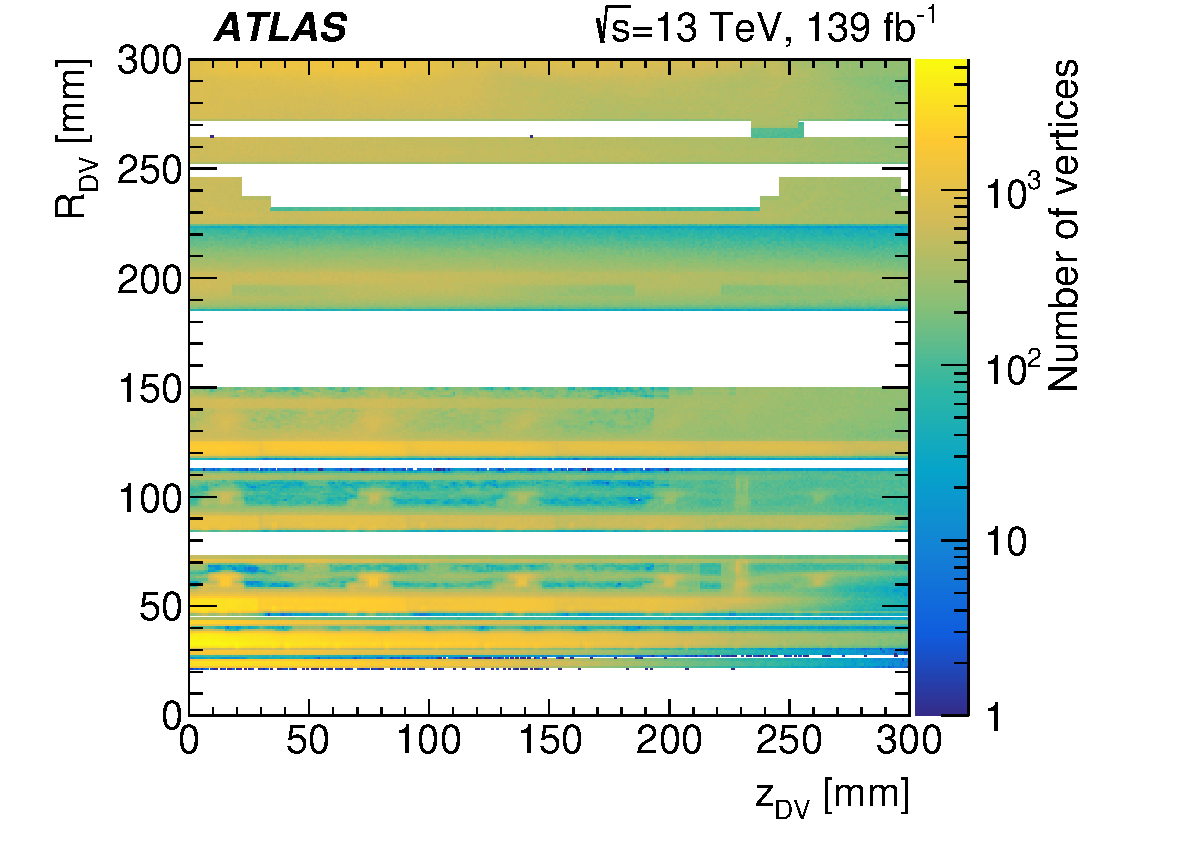
\includegraphics[width=0.5\textwidth]{figures/analysis_strategy/mat_map_rz.pdf}}
        \caption{The positions of reconstructed displaced vertices that are vetoed by the material map.~\cite{SUSY-2018-13}}
        \label{fig:material_map}
    \end{figure}

    \item Cosmic muons: Even though ATLAS is 100 m below the ground, the open shaft above it allows a large flux of muons from the the interaction of cosmic rays with the atmosphere to enter the detector. One such cosmic muon passing through the ATLAS ID can be incorrectly reconstructed as two tracks, with them together reconstructed as the two legs of one secondary vertex. Such a DV is characterized by \textit{back-to-back} tracks i.e. $\eta_\mathrm{track1}\approx-\eta_\mathrm{track2}$ and $\phi_\mathrm{track1}-\phi_\mathrm{track2}\approx\pi$. Hence, a cut on the cosmic separation variable, $\sqrt{(\Sigma_\text{DV tracks}\eta)^2+(\pi-|\Delta_\text{DV tracks}\phi|)^2}>.05$, is applied to reject this background. The exact cut value was optimized for the 2022 analysis, and was found to be sufficient for rejecting all background without affecting signal.

    \item $Z\to\ell\ell$ decays: One of the leptons from a $Z$ decay can be paired with a third uncorrelated lepton to give a lepton+DV topology probed in this analysis. To reject this background, a veto on the $m_{\ell\ell}$ variable around the $Z$ mass, $|m_{\ell\ell}-90\text{ GeV}|>10\text{ GeV}$ is applied to same-flavor opposite-sign (SFOS) pairs of leptons, where one is a prompt lepton and the other is a DV lepton.
\end{enumerate}

~\Cref{tab:cuts_reducible} summarize the cuts applied to reject the three reducible backgrounds that affect this analysis.

\begin{table}[!ht]
    \centering
    \begin{tabular}{cc}
        \hline\hline
         Cut Name & Cut Description\\
         \hline
         Photon Conversions Veto & Material veto applied to $ee$ DVs\\
         Low Mass DV Veto & $\mdv>500$~MeV for $ee$ DVs\\
         Cosmic Muon Veto & $\sqrt{(\Sigma_\text{DV tracks}\eta)^2+(\pi-|\Delta_\text{DV tracks}\phi|)^2}>.05$\\
         $Z\to\ell\ell$ Veto & $|m_{\ell_\mathrm{DV}\ell_\mathrm{prompt}}-90\text{ GeV}|>10\text{ GeV}$ for SFOS pairs \\
         \hline\hline
    \end{tabular}
    \caption{Analysis cuts applied to reject reducible background.}
    \label{tab:cuts_reducible}
\end{table}

\subsection{Irreducible backgrounds}

\begin{figure}[!ht]
    \centering
     \subfloat[Correlated background]{\includegraphics[width=0.4\textwidth]{figures/analysis_strategy/bkg_illustrations/hadrons.png}}
     \subfloat[Uncorrelated background]{\includegraphics[width=0.4\textwidth]{figures/analysis_strategy/bkg_illustrations/crossings.png}}
     \caption{Illustrative topology of the irreducible backgrounds in the ATLAS ID volume.}
     \label{fig:bkg_irreducible}
\end{figure}

Two sources of irreducible backgrounds affect this analysis, as illustrated in~\cref{fig:bkg_irreducible}:
\begin{enumerate}
    \item Correlated background: The largest background that affects this analysis is the lepton+DV signature coming from correlated decay sources. Heavy hadrons, such as b-hadrons and secondary $J/\psi$, mimic signatures from BSM LLPs and decay macroscopically in the ID volume. While these decays are often multi-legged, two of its legs can be captured by VSI and hence contaminate the phase space targeted in this analysis.~\Cref{sec:corr_bkg} describes the detailed study of this background and the method of its estimation.

    \item Uncorrelated background: A (non-)negligible background contribution comes in the form of uncorrelated track pairs, or \textit{random crossings} (RC), that happen to cross in an event and then captured by VSI. The DV is not a genuine decay but rather an accidental point of crossing.~\Cref{sec:uncorr_bkg} describes the method used in the analysis to estimate the contribution from random crossing background.
\end{enumerate}

\section{Correlated Background}\label{sec:corr_bkg}
As previously stated, the biggest background in this analysis is the background from the production of heavy flavor (HF) hadrons which decay to leptons that are displaced with respect to the primary vertex. These are predominantly found in the \mdv$<5$~GeV phase space. Such a phase space was completely removed from consideration in the 2022 analysis due to the lack of a robust method to estimate them which significantly reduced sensitivity to low mass HNLs. In this analysis, MC simulations of SM processes (specifically of the $t\bar{t}$ and $V+$jets processes) are used to understand and estimate this background. A signal rich phase space, called the Signal Region (SR), is defined to look for HNLs in a wide lifetime-coupling parameter space. A non-overlapping phase space rich in correlated background, called the Heavy Flavor Control Region (HF-CR), is defined to estimate the contribution of this background in a data-driven manner.

\subsection{Analysis regions}

All events considered in this analysis are required to have at least one primary vertex with two tracks with \pT$>500$~MeV. The hard-scatter vertex is selected among all reconstructed primary vertices as the one with the largest $\Sigma\pT^2$, where the sum is over all the tracks attached to the PV.

A pre-selection cut is applied for the selection of signatures from a $W$-decay. The tri-lepton invariant mass ($m_{\ell\ell\ell}$) is used as a proxy for the $W$ mass. Events are required to have 40 GeV$<m_{\ell\ell\ell}<$90 GeV, where the lower cut is more liberal compared to the upper cut to account for energy losses from a neutrino emission. A $J/\psi$-veto is applied for $ee$ and $\mu\mu$ DVs requiring $|\mdv-3.1\text{ GeV}|>0.1\text{ GeV}$.

The final pre-selection cut is applied using a discriminating variable optimized to significantly suppress the contribution from hadron decays. The variable $\mathcal{S}$ is defined as
\begin{equation}
    \mathcal{S}^{2} = {\boldsymbol{\Delta}_{\text{3D}}\text{(PV,DV)}}^T \cdot  {\text{\textbf{Cov}}(\Delta_{\text{3D}(\text{PV,DV})})^{-1}} \cdot {\boldsymbol{\Delta}_{\text{3D}}\text{(PV,DV)}},
\end{equation}
where $\boldsymbol{\Delta}_{\text{3D}}\text{(PV,DV)}$ is the 3D vector of the distance between the primary- and secondary-vertex position, and $\text{\textbf{Cov}}(\Delta_{\text{3D}(\text{PV,DV})})$ is the covariance matrix of the difference between the primary- and secondary-vertex position. $\mathcal{S}$ can be interpreted as a significance of the the PV-DV distance. 
%Effectively, this is implemented as follows, defining $\mathcal{W} = \text{Cov}(\Delta_{\text{3D}}(\text{PV,DV}))^{-1}$,
%\begin{equation}
%     \mathcal{S}^{2} = \Delta X^{2} \cdot \mathcal{W}_{00} + \Delta Y^{2} \cdot \mathcal{W}_{11} + \Delta Z^{2} \cdot \mathcal{W}_{22} + 2\Delta X \Delta Y \cdot\mathcal{W}_{01} + 2\Delta X \Delta Z \cdot\mathcal{W}_{02} + 2\Delta Y \Delta Z \cdot\mathcal{W}_{12},
% \end{equation}
%where $\Delta X = \text{PV}_{x} - \text{DV}_{x}$, $\Delta Y$ and $\Delta Z$ are defined in the same way. 
Roughly speaking, DVs with lower values of $\mathcal{S}$ have larger $\pT^\text{DV tracks}$ and lower \rdv and $\Delta R$ between the DV tracks.
 
\begin{figure}[!ht]
    \centering
    \subfloat[Hadron decay background]{\includegraphics[width=0.45\textwidth]{figures/analysis_strategy/S2D_bkg.pdf}}\\
    \subfloat[\mhnl=2 GeV, \ctau=1000 mm HNL signal]{\includegraphics[width=0.45\textwidth]{figures/analysis_strategy/S2D_HNL2_ctau1000.pdf}}
    \subfloat[\mhnl=7.5 GeV, \ctau=100 mm HNL signal]{\includegraphics[width=0.45\textwidth]{figures/analysis_strategy/S2D_HNL7p5_ctau100.pdf}}
    \caption{Distribution of events as a function of the $\mathcal{S}$ variable, referred to as `DV significance' in the plots and \mdv.}
    \label{fig:dvsigni_MDV}
\end{figure}

The distribution of events as a function of $\mathcal{S}$ and the mass of the displaced vertex, $m_{\text{DV}}$ is shown in \cref{fig:dvsigni_MDV} for the hadron decay background predicted by the combination of $t\bar{t}$ and $V+$jets MC simulations as well as for representative signals in for pairs (\mhnl, \ctau) = (2 GeV, 1000 mm) and (7.5 GeV, 100 mm).

From~\cref{fig:dvsigni_MDV}, it is clear that the hadron decay backgrounds are characterised by lower values of $\mathcal{S}$, while for the signal samples the discriminant variable peaks at values above 100. Furthermore, the events from the SM processes are present only for displaced vertices masses below 5 GeV, as they are mostly produced in $B$-hadron decay chains. For this reasons, I decided to apply the following selection to all the events in the analysis: $\mathcal{S}>100$ \textit{if} \mdv$<5$~GeV. This means that all the events outside of the rectangle defined by the four coordinates (0,0), (5,0), (0,100), (5,100) in the $(\mdv\,[\text{GeV}],\mathcal{S})$ plane are retained.

The SR is defined by requiring, on top of the events pre-selection, that the two displaced leptons satisfy an isolation criterion, using the \texttt{Loose\_VarRad}~\cite{EGAM-2018-01} WP for electrons, and the \texttt{PflowLoose\_VarRad} WP~\cite{MUON-2018-03} for muons. Leptons from the DV tend to be collimated and hence close-by-effects\footnote{The calculation of isolation variables uses low-level information from the tracker and the calorimeter without relying on object-level reconstruction. When two leptons are close to each other, they will contribute to the calculation of each other's isolation variables. However, since isolation is only supposed to identify leptons in jets, such a lepton-close-by-effect is an artefact of the method and needs to be corrected.} that might appear in the evaluation of isolation variables are taken into account and correctly subtracted from both the track term and the calorimeter term that define the isolation working points. This procedure is done since Run-1 in $H\to ZZ^*\to 4\ell$ analyses, and generally applies to boosted multi-lepton signatures utilizing lepton isolation. The HF-CR, on the other hand, is defined adding a requirement of at least one non-isolated displaced lepton. To further suppress signal contamination in this region, at least one b-tagged jet is required. This requirement does not bias the kinematics of the correlated background in the HF-CR away from the SR. Lastly, since this analysis probes HNLs with masses up to 20 GeV, the phase space beyond \mhnl$>20$~GeV is not considered in the SR. ~\Cref{tab:sr_cr_cuts} summarizes the cuts used for the SR and the HF-CR. There are 6 SRs and 6 HF-CRs defined in this analysis, one each per channel.

\begin{table}[!ht]
    \centering
    %\begin{tabularx}{\textwidth}{*{3}{>{\centering\arraybackslash}X}}
    \resizebox{\columnwidth}{!}{
    \begin{tabular}{>{\centering}p{0.4\textwidth-70pt}
                    >{\centering}p{0.3\textwidth}
                    cp{0.3\textwidth-220pt}}
         \hline\hline
         Cut Name &  \multicolumn{2}{c}{Cut Description} \\
         \hline
         \multicolumn{3}{c}{\textbf{Object Selection}} \\
         \hline
         Primary Vertex &  \multicolumn{2}{c}{Largest $\Sigma_\mathrm{tracks} \pT^2$} \\
         Prompt Lepton &  \multicolumn{2}{c}{see~\cref{tab:plep_selection}} \\
         Trigger & \multicolumn{2}{c}{see~\cref{tab:triggers}} \\
         Displaced Lepton &  \multicolumn{2}{c}{see~\cref{tab:disp_muon_selection,tab:disp_electron_selection}} \\
         Overlap Removal &  \multicolumn{2}{c}{see~\cref{tab:overlap_removal}} \\
         Displaced Vertex &  \multicolumn{2}{c}{see~\cref{tab:dv_selection}} \\
         \hline
         \multicolumn{3}{c}{\textbf{Pre-selection}} \\
         \hline
         $\gamma\to e e$ Veto & \multicolumn{2}{c}{Material veto, $|z|<300$~mm and $\mdv>500$~MeV for $ee$ DVs} \\
         Cosmic Muon Veto & \multicolumn{2}{c}{$\sqrt{(\Sigma_\text{DV tracks}\eta)^2+(\pi-|\Delta_\text{DV tracks}\phi|)^2}>.05$}\\
         $Z\to\ell\ell$ Veto & \multicolumn{2}{c}{$|m_{\ell_\mathrm{DV}\ell_\mathrm{prompt}}-90\text{ GeV}|>10\text{ GeV}$ for SFOS pairs} \\
         $W$-decay Selection & \multicolumn{2}{c}{40 GeV $<m_{\ell\ell\ell}<90$ GeV} \\
         $J/\psi$ Veto & \multicolumn{2}{c}{$|\mdv-3.1\text{ GeV}|>0.1\text{ GeV}$ for $ee$ and $\mu\mu$ DVs} \\
         Discriminant & \multicolumn{2}{c}{$\mathcal{S}>100$ \textit{if} \mdv$<5$~GeV} \\
         \hline
         \multicolumn{3}{c}{\textbf{Region Specific Cuts}} \\
         \hline
         & \textbf{SR} & \textbf{HF-CR} \\
         \hline
         DV Lepton Isolation & Both isolated & $\geq 1$ non-isolated \\
         b-jets & - & $\geq 1$ \\
         \mhnl Limit & $<20$~GeV & - \\
         \hline\hline
    %\end{tabularx}
    \end{tabular}
    }
    \caption{Object selection, pre-selection, and other additional cuts used to define the non-overlapping Signal Region and the Heavy Flavor Control Region.}
    \label{tab:sr_cr_cuts}
\end{table}

~\Cref{fig:cr_plots_uuu,fig:cr_plots_uue,fig:cr_plots_uee,fig:cr_plots_euu,fig:cr_plots_eeu,fig:cr_plots_eee} show representative kinematics of important properties of the DV in the event and the tracks in it, the prompt lepton, and the $\mathcal{S}$ discriminant variable for events in the HF-CR for all the six channels.

\begin{figure}[!ht]
    \centering
    \subfloat[{\mdv [GeV]}]{\includegraphics[width=0.24\linewidth]{figures/analysis_strategy/CR_plots/uuu/DV_mass.pdf}}
    \subfloat[{$r_\mathrm{DV}$ [mm]}]{\includegraphics[width=0.24\linewidth]{figures/analysis_strategy/CR_plots/uuu/DV_r.pdf}}
    \subfloat[{$\mathcal{S}$}]{\includegraphics[width=0.24\linewidth]{figures/analysis_strategy/CR_plots/uuu/DV_distFromPVsigni.pdf}}
    \subfloat[{prompt lep. \pT [GeV]}]{\includegraphics[width=0.24\linewidth]{figures/analysis_strategy/CR_plots/uuu/prompt_lepton_pt.pdf}}\\
    \subfloat[{$\Delta R$ DV tracks}]{\includegraphics[width=0.24\linewidth]{figures/analysis_strategy/CR_plots/uuu/DV_track_dR.pdf}}
    \subfloat[{\pT of DV tracks [GeV]}]{\includegraphics[width=0.24\linewidth]{figures/analysis_strategy/CR_plots/uuu/DV_trk_pt.pdf}}
    \subfloat[{$\eta$ of DV tracks}]{\includegraphics[width=0.24\linewidth]{figures/analysis_strategy/CR_plots/uuu/DV_trk_eta.pdf}}
    \subfloat[{$d_0$ of DV tracks [mm]}]{\includegraphics[width=0.24\linewidth]{figures/analysis_strategy/CR_plots/uuu/DV_trk_d0.pdf}}
    \caption{Representative kinematics of the displaced vertex, tracks in the displaced vertex, and of the prompt lepton measured in ATLAS data and modeled by MC simulations in the \uuu Heavy Flavor Control Region.}
    \label{fig:cr_plots_uuu}
\end{figure}

\begin{figure}[!ht]
    \centering
    \subfloat[{\mdv [GeV]}]{\includegraphics[width=0.24\linewidth]{figures/analysis_strategy/CR_plots/uue/DV_mass.pdf}}
    \subfloat[{$r_\mathrm{DV}$ [mm]}]{\includegraphics[width=0.24\linewidth]{figures/analysis_strategy/CR_plots/uue/DV_r.pdf}}
    \subfloat[{$\mathcal{S}$}]{\includegraphics[width=0.24\linewidth]{figures/analysis_strategy/CR_plots/uue/DV_distFromPVsigni.pdf}}
    \subfloat[{prompt lep. \pT [GeV]}]{\includegraphics[width=0.24\linewidth]{figures/analysis_strategy/CR_plots/uue/prompt_lepton_pt.pdf}}\\
    \subfloat[{$\Delta R$ DV tracks}]{\includegraphics[width=0.24\linewidth]{figures/analysis_strategy/CR_plots/uue/DV_track_dR.pdf}}
    \subfloat[{\pT of DV tracks [GeV]}]{\includegraphics[width=0.24\linewidth]{figures/analysis_strategy/CR_plots/uue/DV_trk_pt.pdf}}
    \subfloat[{$\eta$ of DV tracks}]{\includegraphics[width=0.24\linewidth]{figures/analysis_strategy/CR_plots/uue/DV_trk_eta.pdf}}
    \subfloat[{$d_0$ of DV tracks [mm]}]{\includegraphics[width=0.24\linewidth]{figures/analysis_strategy/CR_plots/uue/DV_trk_d0.pdf}}
    \caption{Representative kinematics of the displaced vertex, tracks in the displaced vertex, and of the prompt lepton measured in ATLAS data and modeled by MC simulations in the \uue Heavy Flavor Control Region.}
    \label{fig:cr_plots_uue}
\end{figure}

\begin{figure}[!ht]
    \centering
    \subfloat[{\mdv [GeV]}]{\includegraphics[width=0.24\linewidth]{figures/analysis_strategy/CR_plots/uee/DV_mass.pdf}}
    \subfloat[{$r_\mathrm{DV}$ [mm]}]{\includegraphics[width=0.24\linewidth]{figures/analysis_strategy/CR_plots/uee/DV_r.pdf}}
    \subfloat[{$\mathcal{S}$}]{\includegraphics[width=0.24\linewidth]{figures/analysis_strategy/CR_plots/uee/DV_distFromPVsigni.pdf}}
    \subfloat[{prompt lep. \pT [GeV]}]{\includegraphics[width=0.24\linewidth]{figures/analysis_strategy/CR_plots/uee/prompt_lepton_pt.pdf}}\\
    \subfloat[{$\Delta R$ DV tracks}]{\includegraphics[width=0.24\linewidth]{figures/analysis_strategy/CR_plots/uee/DV_track_dR.pdf}}
    \subfloat[{\pT of DV tracks [GeV]}]{\includegraphics[width=0.24\linewidth]{figures/analysis_strategy/CR_plots/uee/DV_trk_pt.pdf}}
    \subfloat[{$\eta$ of DV tracks}]{\includegraphics[width=0.24\linewidth]{figures/analysis_strategy/CR_plots/uee/DV_trk_eta.pdf}}
    \subfloat[{$d_0$ of DV tracks [mm]}]{\includegraphics[width=0.24\linewidth]{figures/analysis_strategy/CR_plots/uee/DV_trk_d0.pdf}}
    \caption{Representative kinematics of the displaced vertex, tracks in the displaced vertex, and of the prompt lepton measured in ATLAS data and modeled by MC simulations in the \uee Heavy Flavor Control Region.}
    \label{fig:cr_plots_uee}
\end{figure}

\begin{figure}[!ht]
    \centering
    \subfloat[{\mdv [GeV]}]{\includegraphics[width=0.24\linewidth]{figures/analysis_strategy/CR_plots/euu/DV_mass.pdf}}
    \subfloat[{$r_\mathrm{DV}$ [mm]}]{\includegraphics[width=0.24\linewidth]{figures/analysis_strategy/CR_plots/euu/DV_r.pdf}}
    \subfloat[{$\mathcal{S}$}]{\includegraphics[width=0.24\linewidth]{figures/analysis_strategy/CR_plots/euu/DV_distFromPVsigni.pdf}}
    \subfloat[{prompt lep. \pT [GeV]}]{\includegraphics[width=0.24\linewidth]{figures/analysis_strategy/CR_plots/euu/prompt_lepton_pt.pdf}}\\
    \subfloat[{$\Delta R$ DV tracks}]{\includegraphics[width=0.24\linewidth]{figures/analysis_strategy/CR_plots/euu/DV_track_dR.pdf}}
    \subfloat[{\pT of DV tracks [GeV]}]{\includegraphics[width=0.24\linewidth]{figures/analysis_strategy/CR_plots/euu/DV_trk_pt.pdf}}
    \subfloat[{$\eta$ of DV tracks}]{\includegraphics[width=0.24\linewidth]{figures/analysis_strategy/CR_plots/euu/DV_trk_eta.pdf}}
    \subfloat[{$d_0$ of DV tracks [mm]}]{\includegraphics[width=0.24\linewidth]{figures/analysis_strategy/CR_plots/euu/DV_trk_d0.pdf}}
    \caption{Representative kinematics of the displaced vertex, tracks in the displaced vertex, and of the prompt lepton measured in ATLAS data and modeled by MC simulations in the \euu Heavy Flavor Control Region.}
    \label{fig:cr_plots_euu}
\end{figure}

\begin{figure}[!ht]
    \centering
    \subfloat[{\mdv [GeV]}]{\includegraphics[width=0.24\linewidth]{figures/analysis_strategy/CR_plots/eeu/DV_mass.pdf}}
    \subfloat[{$r_\mathrm{DV}$ [mm]}]{\includegraphics[width=0.24\linewidth]{figures/analysis_strategy/CR_plots/eeu/DV_r.pdf}}
    \subfloat[{$\mathcal{S}$}]{\includegraphics[width=0.24\linewidth]{figures/analysis_strategy/CR_plots/eeu/DV_distFromPVsigni.pdf}}
    \subfloat[{prompt lep. \pT [GeV]}]{\includegraphics[width=0.24\linewidth]{figures/analysis_strategy/CR_plots/eeu/prompt_lepton_pt.pdf}}\\
    \subfloat[{$\Delta R$ DV tracks}]{\includegraphics[width=0.24\linewidth]{figures/analysis_strategy/CR_plots/eeu/DV_track_dR.pdf}}
    \subfloat[{\pT of DV tracks [GeV]}]{\includegraphics[width=0.24\linewidth]{figures/analysis_strategy/CR_plots/eeu/DV_trk_pt.pdf}}
    \subfloat[{$\eta$ of DV tracks}]{\includegraphics[width=0.24\linewidth]{figures/analysis_strategy/CR_plots/eeu/DV_trk_eta.pdf}}
    \subfloat[{$d_0$ of DV tracks [mm]}]{\includegraphics[width=0.24\linewidth]{figures/analysis_strategy/CR_plots/eeu/DV_trk_d0.pdf}}
    \caption{Representative kinematics of the displaced vertex, tracks in the displaced vertex, and of the prompt lepton measured in ATLAS data and modeled by MC simulations in the \eeu Heavy Flavor Control Region.}
    \label{fig:cr_plots_eeu}
\end{figure}

\begin{figure}[!ht]
    \centering
    \subfloat[{\mdv [GeV]}]{\includegraphics[width=0.24\linewidth]{figures/analysis_strategy/CR_plots/eee/DV_mass.pdf}}
    \subfloat[{$r_\mathrm{DV}$ [mm]}]{\includegraphics[width=0.24\linewidth]{figures/analysis_strategy/CR_plots/eee/DV_r.pdf}}
    \subfloat[{$\mathcal{S}$}]{\includegraphics[width=0.24\linewidth]{figures/analysis_strategy/CR_plots/eee/DV_distFromPVsigni.pdf}}
    \subfloat[{prompt lep. \pT [GeV]}]{\includegraphics[width=0.24\linewidth]{figures/analysis_strategy/CR_plots/eee/prompt_lepton_pt.pdf}}\\
    \subfloat[{$\Delta R$ DV tracks}]{\includegraphics[width=0.24\linewidth]{figures/analysis_strategy/CR_plots/eee/DV_track_dR.pdf}}
    \subfloat[{\pT of DV tracks [GeV]}]{\includegraphics[width=0.24\linewidth]{figures/analysis_strategy/CR_plots/eee/DV_trk_pt.pdf}}
    \subfloat[{$\eta$ of DV tracks}]{\includegraphics[width=0.24\linewidth]{figures/analysis_strategy/CR_plots/eee/DV_trk_eta.pdf}}
    \subfloat[{$d_0$ of DV tracks [mm]}]{\includegraphics[width=0.24\linewidth]{figures/analysis_strategy/CR_plots/eee/DV_trk_d0.pdf}}
    \caption{Representative kinematics of the displaced vertex, tracks in the displaced vertex, and of the prompt lepton measured in ATLAS data and modeled by MC simulations in the \eee Heavy Flavor Control Region.}
    \label{fig:cr_plots_eee}
\end{figure}

\subsection{Truth classification}
As previously mentioned, the kinematics of the hadron decay background are modeled using MC simulations of $t\bar{t}$ and $V+$jets processes and the normalization is obtained from data. Other processes, such as di-boson, multi-jet, $b\bar{b}$, which could lead to the considered final state were studied, and the contribution from them was found to be negligible. Such simulations offer a way to study the physical source of the final state using the \textit{truth origin}\footnote{The truth origin of a track, an integer value ranging from 0 to 45, demarcates the nature of the particle which decayed to give the DV track using the \texttt{MCTruthClassifier}~\cite{mc-truth-web} package. The available categories can be seen in the ATLAS reconstruction framework \url{https://gitlab.cern.ch/atlas/athena/-/blob/24.0/PhysicsAnalysis/MCTruthClassifier/MCTruthClassifier/MCTruthClassifierDefs.h}.}. 
of the tracks in the DV. The truth origin is calculated by looking at the parent information of the truth-matched particle of an ID track. Based on the kind of the parent, the truth origin is dilineated into a set of categories.

\begin{figure}[!ht]
    \centering
    \includegraphics[width=0.66\linewidth]{figures/analysis_strategy/mc_classifier_studies/truth_classification_example.pdf}
    \caption{Event categories based on the truth classification of tracks associated to the displaced vertex in the control region of the \uuu channel for the total MC background.}
    \label{fig:mctruth_groups}
\end{figure}

In ~\cref{fig:mctruth_groups}, an example plot shows the grouping of different kind of DVs shown for the events passing the HF-CR selection of the \uuu channel. This region has been chosen because it is a high-statistics region and it allows to clearly highlight the different contributions. The truth origin of one of the two tracks in the DV is plotted on the $x$-axis and the truth origin of the other one is plotted on the $y$-axis. As can be seen from the $z$-axis scale, the two main contribution of the total background are events with truth origins for (track 1, track 2) = (25,26) and (26, 25): these correspond to tracks associated to the decay productions of $B$- (26) and $D$-mesons (25). This is because $B$ mesons can decay into $D$ mesons plus a charged lepton. Subsequently, real leptons can also be produced in multiple steps of the $D$-meson decay-chain. Such cases are reconstructed as a single DV with two charged leptons, thus passing the selection of the analysis. The presence of additional (low quality) tracks in the decay chain are less likely to be captured by the vertexing algorithm, since the track attachment step is modified to only use tracks that pass the track seeding requirements.

Apart from the main source of HF background, some events are also found with one of the tracks having truth origin 23 or 24, corresponding to leptons originating from light hadrons or strange mesons, respectively. These can be found in the decay chains of $B$ and $D$ mesons as well. 

Another non negligible component comes from pairs of track with true origin equal to 27: these are tracks associated to the production of $c\bar{c}$ mesons, i.e. $J/\psi$ contribution. This is suppressed by the $J/\psi$ veto introduced in this round of the analysis, however it still contributes and is localised in the $m_{DV}$ distribution around 3.1 GeV.

Additional background is found to be associated to the production of heavy flavour baryons, both containing $b$- and $c$- quarks. This population of events leads to DVs in which the tracks are classified as coming from bottom meson + charm hadron or charm meson + bottom hadron. 

The last population, significantly smaller than the ones above, consist of events in which at least one the tracks associated to the displaced vertex comes from an unknown (0) origin. This reflects the presence of real $B$- or $D$-meson production which undergo subsequent decays into leptons, with the other lepton comes from either jets in the events located close to the lepton, or, less likely, directly from the underlying event or a pileup track. This category of events is negligible with respect to the others.

A very minor contribution comes from two tracks with truth origin 9, corresponding to tracks associated to the decay of $\tau$ leptons. This component is also negligible and hence ignored in the rest of the analysis.

The population of events at (0,0) is instead cases in which two uncorrelated tracks crossing and producing a secondary vertex. These events will not be taken from the MC simulated samples. Instead, a dedicated estimate of this background is performed, as is outlined in~\cref{sec:uncorr_bkg}.

Given the grouping of the events discussed above, the following two categories are defined:
\begin{enumerate}
    \item Heavy Flavour hadron production: all the events that have as truth origin of at least one track either $b$- or $c$-meson or baryon and the events that have the 27 as the truth origin of both tracks, which corresponds to $c\bar{c}$ meson production,
    \item \textit{other}: rest of the events. This category has a minor contribution and has been considered only for \textit{in itinere} data/MC plots.
\end{enumerate}

The residual contribution of the \textit{other} component, \textbf{not included in the fit templates}, is expected to be mostly covered by the random crossing background estimate, and eventually absorbed by a global MC normalisation factor which will be used to correct the prediction of the HF background component using data in the dedicated control regions.

\begin{figure}[!ht]
    \centering
    \subfloat[SR \uuu]{\includegraphics[width=0.32\textwidth]{figures/analysis_strategy/mc_classifier_studies/SR_uuu.pdf}}
    \subfloat[SR \uue]{\includegraphics[width=0.32\textwidth]{figures/analysis_strategy/mc_classifier_studies/SR_uue.pdf}}
    \subfloat[SR \uee]{\includegraphics[width=0.32\textwidth]{figures/analysis_strategy/mc_classifier_studies/SR_uee.pdf}}\\
    \subfloat[SR \euu]{\includegraphics[width=0.32\textwidth]{figures/analysis_strategy/mc_classifier_studies/SR_euu.pdf}}
    \subfloat[SR \eeu]{\includegraphics[width=0.32\textwidth]{figures/analysis_strategy/mc_classifier_studies/SR_eeu.pdf}}
    \subfloat[SR \eee]{\includegraphics[width=0.32\textwidth]{figures/analysis_strategy/mc_classifier_studies/SR_eee.pdf}}
    \caption{Truth origin distributions of track pairs associated to displaced vertices in the six leptonic signal region channels for the total MC background.}
    \label{fig:truth_origin_SR}
\end{figure}

~\Cref{fig:truth_origin_SR} shows the truth origin distribution for the total MC prediction for the SRs in the six channels. The background composition is very similar to that in the \uuu HF-CR, with the production of heavy-flavour hadrons being the leading contribution. One notable difference between the \uuu HF-CR, discussed previously, and the SR, discussed here, is that there are almost no events with tracks with unknown truth origin (0). This is related to the fact that in the signal regions the two reconstructed leptons matched to the tracks associated to the DV are required to be isolated. Such a requirement reduces the probability that one real lepton produced in a DV is associated to a random track coming from a jet close-by.

\begin{figure}[!ht]
    \centering
    \subfloat[HF-CR \uuu]{\includegraphics[width=0.32\textwidth]{figures/analysis_strategy/mc_classifier_studies/CR_SM_uuu.pdf}}
    \subfloat[HF-CR \uue]{\includegraphics[width=0.32\textwidth]{figures/analysis_strategy/mc_classifier_studies/CR_SM_uue.pdf}}
    \subfloat[HF-CR \uee]{\includegraphics[width=0.32\textwidth]{figures/analysis_strategy/mc_classifier_studies/CR_SM_uee.pdf}}\\
    \subfloat[HF-CR \euu]{\includegraphics[width=0.32\textwidth]{figures/analysis_strategy/mc_classifier_studies/CR_SM_euu.pdf}}
    \subfloat[HF-CR \eeu]{\includegraphics[width=0.32\textwidth]{figures/analysis_strategy/mc_classifier_studies/CR_SM_eeu.pdf}}
    \subfloat[HF-CR \eee]{\includegraphics[width=0.32\textwidth]{figures/analysis_strategy/mc_classifier_studies/CR_SM_eee.pdf}}
    \caption{Truth origin distributions of track pairs associated to displaced vertices in the six leptonic control region channels for the total MC background.}
    \label{fig:truth_origin_CR}
\end{figure}

\begin{comment}
~\Cref{fig:truth_origin_CR} shows the truth origin distribution for the total MC prediction for the SRs in the six channels. The background compositions are similar in the HF-CRs across all six channels as well as to the SRs, with the production of heavy-flavour hadrons being the leading contribution. The presence of a minor component of events categorised as production of heavy-flavour baryons is related to the fact that, in the HF-CRs, at least one of the two displaced leptons is required to be non-isolated.

{\color{red}
\begin{figure}[!ht]
    \centering
    \subfloat[SR \uuu]{\includegraphics[width=0.32\textwidth]{figures/analysis_strategy/mc_classifier_studies/dataMCplots/SR/inclusive_count_of_events_uuu.pdf}}
    \subfloat[SR \uue]{\includegraphics[width=0.32\textwidth]{figures/analysis_strategy/mc_classifier_studies/dataMCplots/SR/inclusive_count_of_events_uue.pdf}}
    \subfloat[SR \uee]{\includegraphics[width=0.32\textwidth]{figures/analysis_strategy/mc_classifier_studies/dataMCplots/SR/inclusive_count_of_events_uee.pdf}}\\
    \subfloat[SR \euu]{\includegraphics[width=0.32\textwidth]{figures/analysis_strategy/mc_classifier_studies/dataMCplots/SR/inclusive_count_of_events_euu.pdf}}
    \subfloat[SR \eeu]{\includegraphics[width=0.32\textwidth]{figures/analysis_strategy/mc_classifier_studies/dataMCplots/SR/inclusive_count_of_events_eeu.pdf}}
    \subfloat[SR \eee]{\includegraphics[width=0.32\textwidth]{figures/analysis_strategy/mc_classifier_studies/dataMCplots/SR/inclusive_count_of_events_eee.pdf}}
    \caption{Inclusive count of events for each of the six leptonic signal regions, divided by the truth classification method. The hatched band represents the MC statistical uncertainty only.}
    \label{fig:truth_origin_SR_inc}
\end{figure}

~\Cref{fig:truth_origin_SR_inc} shows the expected number of events for the signal regions in each of the six channels, diving the MC events based on the truth categories defined previously in this section. As can be seen, the $c\bar{c}$ production component is only present in the channels with SFOS leptons in the DVs. The larger contribution of the \textit{other} component observed in the $x-ee$ channels with respect to $x-x\mu$ channels is due to the difference in identification working points chosen for electrons and muons, with the one for electrons being much looser, thus more subject to be faked by a random track crossing associated to the DV.
These regions (signal regions) are currently blinded.
}

\begin{figure}[!ht]
    \centering
    \subfloat[HF-CR \uuu]{\includegraphics[width=0.32\textwidth]{figures/analysis_strategy/mc_classifier_studies/dataMCplots/CR/inclusive_count_of_events_uuu.pdf}}
    \subfloat[HF-CR \uue]{\includegraphics[width=0.32\textwidth]{figures/analysis_strategy/mc_classifier_studies/dataMCplots/CR/inclusive_count_of_events_uue.pdf}}
    \subfloat[HF-CR \uee]{\includegraphics[width=0.32\textwidth]{figures/analysis_strategy/mc_classifier_studies/dataMCplots/CR/inclusive_count_of_events_uee.pdf}}\\
    \subfloat[HF-CR \euu]{\includegraphics[width=0.32\textwidth]{figures/analysis_strategy/mc_classifier_studies/dataMCplots/CR/inclusive_count_of_events_euu.pdf}}
    \subfloat[HF-CR \eeu]{\includegraphics[width=0.32\textwidth]{figures/analysis_strategy/mc_classifier_studies/dataMCplots/CR/inclusive_count_of_events_eeu.pdf}}
    \subfloat[HF-CR \eee]{\includegraphics[width=0.32\textwidth]{figures/analysis_strategy/mc_classifier_studies/dataMCplots/CR/inclusive_count_of_events_eee.pdf}}
    \caption{Inclusive count of events for each of the six Heavy Flavor Control Regions, divided by the truth classification method. The hatched band represents the MC statistical uncertainty only. The black dots represent ATLAS Run-2 data.}
    \label{fig:truth_origin_CR_inc}
\end{figure}

~\Cref{fig:truth_origin_CR_inc} shows the expected number of events for the HF-CRs in each of the six channels, diving the MC events based on the truth categories defined previously in this section. Also in this case, as for the SR, the $c\bar{c}$ production component is only prevalent in the channels with SFOS displaced leptons. The same comment about the \textit{other} component holds as well. Overall, the total number of events predicted by the MC simulation matches, within uncertainty, to what is observed in data.
\end{comment}

\subsection{Background prediction}
To exploit the fact that the different background components have different DV mass distributions, the chosen variable  in the HF-CRs for the statistical analysis, described later in~\cref{sec:sig_ext}, is \mdv itself. On the other hand, since the HNL signal extraction is done from the SRs, the reconstructed HNL mass (\mhnl) introduced in the 2022 analysis (details of calculation in Appendix A of~\cite{PhysRevLett.131.061803}) is used for its strong discrimination power. The reconstruction uses energy-momentum conservation in the HNL production ($W\to\mathcal{N}\ell_1$) and decay ($\mathcal{N}\to\ell_1\ell_2\nu$) to get around the lack of measurement of the neutrino kinematics. The MC samples are used to build the templates of predictions used in the statistical analysis.~\Cref{fig:mhnl_signal} shows the reconstructed \mhnl for signal samples with various simulated masses and $\ctau = 10$~mm. The \mhnl resolution for channels with $\mu\mu$ DVs is the best, followed by $\mu e$ and $ee$ DVs. This is due to the use of the kinematics of the track object and not of the lepton object in the reconstruction of this variable. Since GSF tracks don't fully account for radiation losses from electrons, they give a worse momentum measurement of the HNL decay products, and hence a worse reconstructed \mhnl value.

\begin{figure}[!ht]
    \centering
    \subfloat[\uuu]{\includegraphics[width=0.32\textwidth]{figures/analysis_strategy/uuu_mHNL.pdf}}
    \subfloat[\uue]{\includegraphics[width=0.32\textwidth]{figures/analysis_strategy/uue_mHNL.pdf}}
    \subfloat[\uee]{\includegraphics[width=0.32\textwidth]{figures/analysis_strategy/uee_mHNL.pdf}}
    \caption{Reconstructed \mhnl distributions for signal samples with $\ctau = 10$~mm. The signals are scaled to arbitrary values for side-by-sde comparison between different mass points.}
    \label{fig:mhnl_signal}
\end{figure}

The available statistics from MC simulations is sufficient in the HF-CRs, therefore, the expected background MC events are used. A systematic uncertainty equal to the relative statistical uncertainty of the background MC predictions is assigned to this template. In the HF predictions in the SR, instead, some un-physical statistical fluctuations are observed. Furthermore, insufficient statistics in the SR from the MC samples lead to no background prediction beyond $\mhnl=7$~GeV. In order to reduce the impact of such artefacts, the shape of the \mhnl distribution of the HF background in the SR is obtained from a shape region (ShR) with requirements on the DV lepton isolation and $m_{\ell\ell\ell}$ removed. Since similar kinematics and compositions are observed in all the regions for this background, events from the ShR of all six channels are combined to obtain the shape. Finally, the shape is scaled back to the event yield predicted by MC simulations in the six individual channels. A dedicated systematic uncertainty is assigned to this method to cover the assumptions made with the details mentioned in~\cref{sec:sig_ext}.
 
\begin{figure}[!ht]
    \centering
    \includegraphics[width=\linewidth]{figures/analysis_strategy/template_building/template_building_SR.pdf}
    \caption{Template building method used for the HF background in the Signal Regions.}
    \label{fig:template_building}
\end{figure}

~\Cref{fig:template_building} shows the template building procedure for the HF background component in the SR. It shows the merging of the six different channels (bottom row), first in \xuu, \xue and \xee channels (middle row), and then all the channels merged (top plot). The yield from ShR in each case is shown, normalized to the nominal MC event yield for a one-to-one shape comparison. The original MC at each level is shown with black dots and the shape from ShR normalized to the origianl MC in individual channels in shown in dashed red lines. For the sake of illustration, the ShR shape at the DV flavor level is also shown in blue, however this shape is not used directly in the analysis. Finally, the shape from the ShR for all channels combined, which is used as the SR background estimate shape in the SR, is shown by the green line. The agreement between the original MC predictions and the ShR shape is sufficiently good across all channels in the $\mhnl=1-7$~GeV range, with the ShR prediction also giving a non-zero prediction in the tails of the distribution, i.e. in the $\mhnl=7-20$~GeV range. The templates obtained with this method are shown in~\cref{fig:templates_hf_sr}. 

\begin{figure}[!ht]
    \centering
    \subfloat[SR \uuu]{\includegraphics[width=0.32\textwidth]{figures/analysis_strategy/template_building/HF_SR_uuu_fitTemplate_MergeDVtype_multiComp.pdf}}
    \subfloat[SR \uue]{\includegraphics[width=0.32\textwidth]{figures/analysis_strategy/template_building/HF_SR_uue_fitTemplate_MergeDVtype_multiComp.pdf}}
    \subfloat[SR \uee]{\includegraphics[width=0.32\textwidth]{figures/analysis_strategy/template_building/HF_SR_uee_fitTemplate_MergeDVtype_multiComp.pdf}}\\
    \subfloat[SR \euu]{\includegraphics[width=0.32\textwidth]{figures/analysis_strategy/template_building/HF_SR_euu_fitTemplate_MergeDVtype_multiComp.pdf}}
    \subfloat[SR \eeu]{\includegraphics[width=0.32\textwidth]{figures/analysis_strategy/template_building/HF_SR_eeu_fitTemplate_MergeDVtype_multiComp.pdf}}
    \subfloat[SR \eee]{\includegraphics[width=0.32\textwidth]{figures/analysis_strategy/template_building/HF_SR_eee_fitTemplate_MergeDVtype_multiComp.pdf}}
    \caption{Comparison of the original MC predictions and different smoothed predictions for the HF background in the Signal Regions.}
    \label{fig:templates_hf_sr}
\end{figure}


\section{Uncorrelated Background}\label{sec:uncorr_bkg}
The Random Crossing background consists of a pair of uncorrelated tracks crossing each other in space and accidentally getting reconstructed as a DV paired with a prompt lepton to yield an event in our measured phase space. These exact characteristics of the RC background are used to estimate them, the method for which was developed for~\cite{Barlow:1749971}.~\Cref{fig:rc_method} illustrates the steps used to create RC DV candidates in a data driven manner.

\begin{figure}[!ht]
    \centering
    \includegraphics[width=\textwidth]{figures/analysis_strategy/random_crossing/rtc_scheme.png}
    \caption{Schematic illustration of track pool creation from different events used to create randomly paired tracks for artificial vertex creation to estimate the random track crossing background.}
    \label{fig:rc_method}
\end{figure}

In the first step, a pool of tracks passing the track selection requirements of VSI is created from all available data events. From this pool, track pairs are randomly selected (with replacement) which are required to come from different events. In the last step, these track pairs are passed through VSI and a DV reconstruction is attempted. The result is a set of artificial DVs representative of the vertices expected to result from random track crossings.

The probability to obtain a DV from a track pair ($p(\text{DV|pair})$) is given by:
\begin{equation}
    p(\text{DV|pair}) \approx \lim_{N_\text{Attempts}\to \infty}\frac{N_\text{DV}}{N_\text{Attempts}}.
\end{equation}
where $N_\text{Attempts}$ is the number of times a DV reconstruction is attempted using track pairs and $N_\text{DV}$ is the number of times a DV was successfully reconstructed in the attempts. The number of predicted RC DVs ($N_\text{Predicted crossings}$), hence, follows as:
\begin{equation}\label{eq:crossings}
    N_\text{Predicted crossings} = p(\text{DV}|\text{Pair}) \times N_\text{Real} = N_{DV} \times \frac{N_\text{Real}}{N_\text{Attempts}}.
\end{equation}
Therefore, each artificially reconstructed RC DV is weighted by a factor $\frac{N_\text{Real}}{N_\text{Attempts}}$, where $N_\text{Real}$ is the number of combinatorial track pairs found in data. Care is taken to ensure that~\cref{eq:crossings} are representative of unrelated track pairs. Correlated track pairs from decaying resonances should not enter $N_\mathrm{Real}$, as such pairs do not occur randomly, and the DV that may result from them are estimated using dedicated other techniques. To ensure this, both $N_\mathrm{Real}$ and $N_\mathrm{Attempts}$ are obtained by counting pairs with $m_\mathrm{Pair}>6$~GeV to reject low-mass hadron decays, and $|\Delta\phi_\mathrm{Pair}|>2.4$ to reject Drell-Yan and resonant $Z$ decay events. In addition, the normalisation is performed separately for events that contain prompt leptons and events that don’t. The normalisation weights are obtained separately for each DV flavor.

Finally, the RC DV candidate is combined with the prompt lepton to yield a complete signature defining the RC background in this search. The kinematics of this 3-lepton system are then used to reconstruct variables that this analysis is sensitive to, such as \mdv and \mhnl.

The kinematics and normalization of the RC estimate are successfully validated in a phase space rich in this background. The $m_{\ell\ell\ell}$ pre-selection is removed, the fiducial volume cut is relaxed ($2\text{ mm}<\rdv<300\text{ mm}$, and an added high \mdv ($>2$~GeV) requirement is imposed. From this phase space, all events passing the SR cuts are veto-ed to define the validation region. The background is found to be extremely suppressed with very low expected yields in all regions, as shown in~\cref{tab:rc_yields}. 

\begin{table}[!htbp]
    \centering
    \begin{tabular}{c|c|c|c|c|c|c|c}
    \hline\hline
        Region & \uuu & \uue & \uee & \euu & \eeu & \eee & Total\\
        \hline
        SR & .025 & .017 & .000 & .002 & .030 & .048 & .123  \\
        HF-CR & .560 & .227 & .044 & .123 & .154 & .380 & 1.489 \\
        \hline \hline
    \end{tabular}
    \caption{Total yields of random crossing backgrounds in the signal and HF control regions for the six channels.}
    \label{tab:rc_yields}
\end{table}


\section{Signal Extraction}\label{sec:sig_ext}
As previously mentioned, six channels are used in this analysis, and a global signal strength is extracted from all channels for each model. Depending on the model being considered, an HNL signal may or may not have contributions in a certain channel. For instance, a $\mu$ only mixing HNL will have events in the \uuu SR, but not in the \euu SR, since the prompt lepton and the displaced leptons have different flavors in the latter. This fact is used to use the SRs in certain channels to help constrain the HF background along with the CRs. Due to the extremely low HF background contribution in the \eee and \uee SRs, they are combined in the fit to an \xee SR.~\Cref{tab:fit_structure} shows the primary use of the SRs and HF-CRs defined in the analysis for each channel considered. This section outlines the uncertainties considered in the analysis and the structure of the statistical analysis used to extract the global signal strength.

%\begin{landscape}
    \begin{table}[!htbp]
        \footnotesize
        \centering
        %\setlength\extrarowheight{6pt}
        \resizebox{\columnwidth}{!}{
        \begin{tabular}{c|c|c|c|c|c|c}
        \hline\hline
           \multirow{2}{*}{Model} & \multicolumn{5}{c|}{Signal Region}  &  Heavy Flavor Control Region\\
           \cline{2-7}
           & \uuu & \uue & \euu & \eeu & \xee & All Channels \\
           \hline
           1SFH($\mu$) & {\color{green} Signal} & {\color{green} Signal} & {\color{red} Background} & {\color{red} Background} &  {\color{green} Signal} &  \multirow{4}{*}{{\color{red} Background}} \\
           %\cline{1-6}
           1SFH($e$) & {\color{red} Background} & {\color{red} Background} &  {\color{green} Signal} &  {\color{green} Signal} & {\color{green} Signal} &  \\
           %\cline{1-6}
           2QDH(IH) & {\color{green} Signal} & {\color{green} Signal} & {\color{green} Signal} & {\color{green} Signal} & {\color{green} Signal} &  \\
           %\cline{1-6}
           2QDH(NH) & {\color{green} Signal} & {\color{green} Signal} & {\color{green} Signal} & {\color{green} Signal} & {\color{green}       Signal} & \\
           \hline \hline
         \end{tabular}
         }
     \caption{A summary of the use of the fit regions defined for the models that are used in the interpretation of the analysis results. {\color{green} Signal} represents when a region is mainly used for signal extraction, and {\color{red} Background} represents when a region is used for constraining the background from Heavy Flavor decays.}
     \label{tab:fit_structure}
\end{table}
%\end{landscape}

\subsection{Uncertainties}
All relevant sources of uncertainties are considered in this analysis which can affect the estimate on the background and signal MC predictions. One standard deviation ($\pm 1 \sigma$) variations are considered for all uncertainties, and are propagated to the statistical fit. The standardization of LRT objects in this version of the analysis allowed for a better understanding of the uncertainties on these objects in close coordination with the Combined Performance (CP) groups. The use of MC simulations for the modeling of HF decay background warranted an inclusion of the theoretical modeling uncertainties on them, which have been estimated using the prescription from the Physics Modeling Group. This section describes all the sources of systematic uncertainties considered in this analysis. The net impact of the systematic uncertainties on the analysis is shown in~\cref{tab:uncertainty}. Systematics are found the be a sub-dominant source of uncertainties and the results are largely dominated by the statistically limited dataset.

\subsection*{Integrated Luminosity}
The LUCID2 detector was used to measure the integrated luminosity collected by ATLAS during Run-2 with a central value of 140.1 pb$^{-1}$ and an error of 0.83\%~\cite{DAPR-2021-01}.

\subsection*{Pileup}
While pileup is modeled in simulation, the simulated collision conditions are not identical to those experienced during the data collection. A centrally managed tool is used to re-weight signal and background MC events and take into account the impact of pileup during the various data periods.

\subsection*{Trigger}
The efficiency of triggering by a muon or an electron in MC is adjusted to that in data by looking at $Z\to\ell\ell$ events. The efficiency calibrations from the CP groups are used to account for these uncertainties on the primary triggering object, which is the prompt lepton in this analysis.

\subsection*{Lepton Momentum}
The momentum of the leptons measured in MC are calibrated for detector conditions using Z and $J/\psi$ decays. The standard CP efficiency calibrations are used for all leptons used in this analysis.

\subsection*{Lepton Reconstruction and Identification}
The muons in this analysis are either standard or LRT, all accepted using the \texttt{Medium} identification WP. For standard muons, the standard CP efficiency calibrations are applied obtained using $Z(J/\psi)$ decays for muon $\pT >(<)\,10$~GeV in a tag and probe analysis~\cite{MUON-2018-03}. 
For LRT muons, the reconstruction and identification efficiencies are studied separately and are measured indirectly. The efficiency to measure a \texttt{Medium} muon can be divided into two factors:
\begin{equation}
    \epsilon\, (\text{Medium }\mu) \approx \epsilon\, (\text{Medium }\mu \,|\,\mathrm{ID}) \times \epsilon (\mathrm{ID}),
\end{equation}
Here, $\epsilon\, (\text{LRT ID})$ is roughly estimated using $K_S\to\pi^+\pi^-$ decays~\cite{IDTR-2021-03}. Furthermore, it is postulated that
\begin{equation}
    \epsilon\, (\text{Medium LRT }\mu \,|\,\text{LRT ID})\approx\epsilon\, (\text{Medium Standard }\mu \,|\,\text{Standard ID}),
\end{equation}
since the MS is \textit{far} from the IP, and hence is insensitive to cm level displacements that come from the difference in Standard and LRT ID track reconstruction. The above two inferences allow for the calibration of LRT muon reconstruction and identification efficiencies using the same $Z$ and $J/\psi$ decays, since $\epsilon\, (\text{Medium Standard }\mu \,|\,\text{Standard ID})$ is measured by the standard tag and probe method with the ID track corrections (i.e. contribution from $\epsilon\, (\text{Standard ID})$) disabled in the measurement.

After studying the above terms, an uncertainty of $1(3)\%$ is applied on LRT muons with $\pT >(<)\,5$~GeV.

A similar decomposition also applies to the reconstruction and identification of electrons, where separate reconstruction efficiencies are calculated for standard and LRT electrons. For the identification criteria, separate efficiencies are applied to the prompt electron and the displaced electron, since they use the \texttt{Medium} and \texttt{VeryLooseNoPix} identification WPs, respectively.

The electron reconstruction efficiency is accounted with a 3\% uncertainty for both the standard and LRT objects. The \texttt{Medium} electron identification efficiency is measured with a 4\% uncertainty, and \texttt{VeryLooseNoPix} electrons are identified with a 5\% uncertainty.

\subsection*{Lepton Isolation}
The CP efficiency calibrations are used on the calibration of the isolation applied on the prompt and displaced muons, while a conservative 2\% uncertainty is applied on the electron isolation efficiency. Since the same working point is applied on standard and LRT objects without modifications, the same uncertainties are applied to both of them.

\subsection*{Flavor Tagging}
Uncertainties from the measurement of the jet energy scale and resolution were found to have no impact on this analysis. The systematic uncertainties from the calibration of the flavor tagging algorithm are considered using the medium reduction scheme, as recommended by the flavor tagging CP group.

\subsection*{Signal Modeling}
In the 2022 analysis, the HNL process was modeled at LO using \textsc{Pythia}, and the MC prediction was attached a modeling uncertainty of $3\% \oplus 5\%$, with the former coming from the measurement of the $W$ production cross section and the latter from the analytical calculation of the HNL branching fraction compared to the prediction from \textsc{MadGraph5}. It was found that the spin correlations of the HNL decay products were not well modeled by \textsc{Pythia}, and a dedicated reweighting procedure was applied to adjust for the same. In this analysis, the predictions are modeled at NLO with the spin correlation well modeled by the MC event generators. Hence, a reduced yet conservative uncertainty of 5\% is considered on the signal prediction.

\subsection*{Random Crossing Modeling}
The random crossing background estimate reuses ID tracks to create a preliminary track pool, which are later used to reconstruct DVs with uncorrelated objects. The statistical correlation coming from such a multi-count is accounted using a bootstrapping~\cite{ATL-PHYS-PUB-2021-011} mechanism. Furthermore, alternate track sampling methods account for uncertainties coming from the bias in the sampling strategy of such tracks. A conservative 50\% uncertainty is applied on the random crossing background estimate to cover the above effects. Given the very small contribution of this background in all the considered regions, this uncertainty is expected to have a negligible effect.

\subsection*{HF Background Modeling}
As described in~\cref{sec:data_mc_samples}, $t\bar{t}$ and $V+$jets MC samples are used to model the background from HF decays. Theoretical uncertainties are evaluated for both of these MC simulations following the recommendations of the ATLAS Physics Modeling Group:
\begin{itemize}
    \item $\mathbf{t\bar{t}}$: Uncertainties are evaluated for the hard scatter generation (or matrix element calculation), parton showering process, QCD scale, modeling of the initial and final state radiations, and the choice of the parton density function.

    The matrix element uncertainty is evaluated using a two-point comparison between the nominal \textsc{Powheg} sample showered with \textsc{Pythia\,8} and a sample generated with an identical configuration except the \texttt{pThard} parameter of \textsc{Powheg} set to 1 instead of the nominal value of 0. The parton shower uncertainty is evaluated using a two-point comparison between the nominal \textsc{Powheg} sample showered with \textsc{Pythia\,8} and \textsc{Herwig,7} showering program.

    QCD scale uncertainty is evaluated using the five-point envelope of the variations of renormalization and factorization scales by factors of 2.0 or 0.5 (removing the cases when both are 0.5, both are 2, and one is 2.0 and the other is 0.5). The initial and final state radiation uncertainties are calculated using the $\pm 1 \sigma$ weights from \textsc{Pythia\,8}. Lastly, the PDF uncertainty is evaluated using the \textsc{NNPDF3.0nlo} variations in the \textsc{Powheg+Pythia\,8} sample as defined in the \texttt{PDF4LHC} recommendations~\cite{Butterworth_2016}.

    \item $\mathbf{V+}$\textbf{jets}: Uncertainties are evaluated for the QCD scale and parton density function choice.

    QCD scale uncertainty is evaluated using the seven-point envelope of the variations of renormalization and factorization scales by factors of 2.0 or 0.5 (removing the cases when both are 0.5 and both are 2). The PDF uncertainty is evaluated in the same manner as for the $t\bar{t}$ samples following the \texttt{PDF4LHC} recommendations.
\end{itemize}
~\Cref{tab:sys_theo} summarizes the theory uncertainties used for the background modeling and the method used to calculate them.

  \begin{table}[!htbp]
  {
    \begin{tabular}{clcc}
      \hline\hline
      Process & Uncertainty & Variations & Method\\
      \hline
      $t\bar{t}$    & Matrix Element & \textsc{Powheg}+\textsc{Pythia\,8} \texttt{pThard}:0,  & Two-point variation\\
      & & \textsc{Powheg}+\textsc{Pythia\,8} \texttt{pThard}:1 & \\
      & Parton Shower & \textsc{Powheg}+\textsc{Pythia\,8},  & Two-point variation\\
      & & \textsc{Powheg}+\textsc{Herwig\,7} & \\
      & Initial State Radiation & Var3cUp, Var3cDown & up down variation \\
      & Final State Radiation & muRfac=2.0, muRfac=0.5 & up down variation \\
      & QCD Scale &  $\mu_R,\,\mu_F\in\{.5,\,1,\,2\}$ & 5-point envelope \\
      & PDF & NNPDF30\_nlo\_as\_0118 & $\sqrt{\frac{1}{N} \sum_i\left(X_i-X_0\right)^2}$\\
      \hline
      $V$+jets & QCD Scale & $\mu_R,\,\mu_F\in\{.5,\,1,\,2\}$ & 7-point envelope \\
      & PDF & NNPDF30\_nlo\_as\_0118 & $\sqrt{\frac{1}{N} \sum_i\left(X_i-X_0\right)^2}$\\
      \hline
      \hline
    \end{tabular}
    }
    \centering
    \caption{Summary of the theoretical systematic uncertainties considered on the background Monte Carlo simulations and their method of evaluation.}
    \label{tab:sys_theo}
  \end{table}

\subsection*{HF Template Building}
As described previously, a dedicated uncertainty is assigned on the template building process of the HF background. It is equal to the Monte Carlo Statistics uncertainty in the HF-CR, since no smoothing or shape building process is applied in those regions. In the SR, a two-point uncertainty comparing the ShR shape from a single channel and the ShR shape from the combination of all channels is applied. Since the shapes are normalized to the MC event yield of individual channels, this is a shape-only effect.

\subsection*{Monte Carlo Statistics}
Lastly, the MC statistics uncertainty is considered on the signal prediction as well coming from the limited statistics considered in the production of the signal MC samples.

\subsection{Simultaneous fit}
A global likelihood minimizing fit is performed to extract a signal strength for each simulated signal point. A likelihood function $\mathcal{L}$ is used to define a global probability density function of this measurement for. The extended likelihood $\mathcal{L}$ consists of a product of likelihood functions ($\mathcal{P}$s) of the SR yield and CR yield. The function is shown without a channel indexing for simplicity, but a global product runs over all five SRs and six CRs considered in the analysis:
\begin{equation}
\label{eqn:likelihood}
    \mathcal{L} = \mathcal{P}( N_{\mathrm{data}}^{\mathrm{SR}}| \mu \cdot N_{\mathrm{signal}}^{\mathrm{SR}} + 
    \mu_{\mathrm{HF}}  \cdot N_{\mathrm{HF}}^{\mathrm{SR}} + N_{\mathrm{RC}}^{\mathrm{SR}} ) \cdot 
    \mathcal{P}(N_{\mathrm{data}}^{\mathrm{CR}} | \mu_{\mathrm{HF}}\cdot N_{\mathrm{HF}}^{\mathrm{CR}} + N_{\mathrm{RC}}^{\mathrm{CR}}) \cdot                                                    \prod_{i=1}^{n_{\theta_i}}\mathrm{N}(\tilde{\theta_i}| \theta_i),
\end{equation}

where $N_{\mathrm{data}}^{\mathrm{SR}}$ and $N_{\mathrm{data}}^{\mathrm{CR}}$ are the numbers of events observed in data in the signal region and the HF control region, respectively, and $N_{\mathrm{signal}}^{\mathrm{SR}}$ is the expected signal yield in the SR. The parameter $\mu$ is the normalization of the signal, and $\mu_{\mathrm{HF}}$ that of the HF background. A signal strength of $\mu=0$ corresponds to a background only hypothesis while $\mu=1$ corresponds the nominal signal plus background (S+B) hypothesis. $N_{\mathrm{HF}}^{\mathrm{SR}}$ and $N_{\mathrm{HF}}^{\mathrm{CR}}$ are the expected numbers of HF background events in the SR and CR, respectively. As previously mentioned, the RC background is taken directly from the data-driven prediction and is represented by $N_{\mathrm{RC}}^{\mathrm{SR}}$ and $N_{\mathrm{RC}}^{\mathrm{CR}}$ in the SR and CR, respectively.  The term $\mathcal{N}$ is a normal function that parameterizes the systematic effect of the type $i$ as a function of a Gaussian constrained nuisance parameter $\theta_i$ and the associated estimate of the corresponding effect $\tilde{\theta_i}$, as mentioned in the previous section. 

The parameter $n_{\theta_i}$ represents the number of nuisance parameters modeling the systematic uncertainties considered in this analysis. The likelihood function $\mathcal{P}$ in the SR and CR are defined as Poisson probability density functions~\cite{Cranmer:1456844} built from binned histograms (also referred to as templates) of \mhnl and \mdv, respectively, using MC events for signal and HF background and a data driven template for the RC background. Bins of 500 MeV from 0 to 20 GeV in \mhnl are used in the SR determined by the \mhnl reconstruction resolution in signal. Similarly, bins of 500 MeV from 0 to 6 GeV in \mdv are used in the CR, since no HF background is observed beyond 6 GeV. The signal and background templates are also functions of the nuisance parameters~\cite{Cranmer:1456844} such that systematic uncertainties can affect the \mhnl or \mdv shapes for the signal process and the HF background whose yields are extracted from the fit and the normalization for the RC background whose yield is fixed to the prediction. This methodology accounts for correlations of systematic uncertainties between signal and background estimates. All systematics considered in the analysis are fully correlated between regions and whichever samples they apply to, expect for the systematics from template building and MC statistics, which are decorrelated between each bin and region. 

The likelihood is maximized to determine the best fit value of the global signal strength $\mu$. More specifically, the profile likelihood is used instead of the likelihood to correctly account for the effect of the systematics near the minimization point, and is given by:
\begin{equation}
    \lambda(\mu) = \frac{\mathcal{L}(\mu,\hat{\hat{\theta_\mu}})}{\mathcal{L}(\hat{\mu},\hat{\theta_\mu})},
\end{equation}
where $\hat{\mu}$ and $\hat{\theta_\mu}$ are estimators for the signal strength and nuisance parameters that maximize the likelihood globally, and $\hat{\hat{\theta_\mu}}$ is a conditional likelihood maximizing estimator for a specific $\mu$. 

The test statistic is built using the profile likelihood ratio which is minimized to determine the best fit value:
\begin{equation}
    q_{\mu} = -2\ln{\lambda(\mu)}.
\end{equation}
The probability of the background fluctuating such that it is equal to larger than the number of data events is given by the p-value $p_0$:
\begin{equation}
    p_0=\int_{q_{\mathrm{obs}}}^{\infty} f\left(q_0 \mid 0, \hat{\theta}_0\right) \mathrm{d} q_0,
\end{equation}
where the integrand is the probability distribution function in the background-only hypothesis $q_0$ and $q_{\mathrm{obs}}$ is the observed test statistic. Similarly, a p-value for the S+B hypothesis $p_{\mu}$ is defined as:
\begin{equation}
    p_\mu=\int_{q_{\mathrm{obs}}}^{\infty} f\left(q_\mu \mid \mu, \hat{\theta}_\mu\right) \mathrm{d} q_\mu.
\end{equation}

The CL$_{s}$~\cite{Read_2002} method is used to exclude signal hypothesis since it has been shown to perform better than a standard p-value based exclusion in analysis of statistically limit datasets. The test statistic is defined as:
\begin{equation}
    \mathrm{CL}_s = \frac{p_\mu}{p_0}.
\end{equation}
The 95\% confidence level (CL) upper limit on the signal strength can be found by varying $\mu$ until CL$_s (\mu_\mathrm{limit})=0.05$. Signal models are excluded if $\mu_{\mathrm{limit}} < 1$.

\Cref{fig:pre_fit_CR} shows the \mdv distribution of measured data, random crossing background, and expected HF background in the six CRs. Good agreement between the data and predictions is observed across all regions within errors in data counting (shown by black lines around data points) and systematic uncertainties (shown by hashed bands around the HF background estimate), with some discrepancies expected to be corrected by the fit.

\begin{figure}[!htbp]
    \centering
    \subfloat[HF-CR \uuu]{\includegraphics[width=0.25\textwidth]{figures/analysis_strategy/pre_fit/CRuuu.pdf}}
    \subfloat[HF-CR \uue]{\includegraphics[width=0.25\textwidth]{figures/analysis_strategy/pre_fit/CRuue.pdf}}
    \subfloat[HF-CR \uee]{\includegraphics[width=0.25\textwidth]{figures/analysis_strategy/pre_fit/CRuee.pdf}}\\
    \subfloat[HF-CR \euu]{\includegraphics[width=0.25\textwidth]{figures/analysis_strategy/pre_fit/CReuu.pdf}}
    \subfloat[HF-CR \eeu]{\includegraphics[width=0.25\textwidth]{figures/analysis_strategy/pre_fit/CReeu.pdf}}
    \subfloat[HF-CR \eee]{\includegraphics[width=0.25\textwidth]{figures/analysis_strategy/pre_fit/CReee.pdf}}
    \caption{Data and pre-fit background \mdv distributions in the six control regions. Inclusive yields shown in the legend are rounded to the first decimal point.}
    \label{fig:pre_fit_CR}
\end{figure}

Similarly,~\cref{fig:pre_fit_SR} shows the \mhnl distributions of measured data and expected backgrounds in the five SRs. A good compatibility is also seen between the background predictions and the observed data, with the exception of a few outlying events, an analysis of which is presented in~\cref{sec:event_excess}.

\begin{figure}[!htbp]
    \centering
    \subfloat[SR \uuu]{\includegraphics[width=0.25\textwidth]{figures/analysis_strategy/pre_fit/SRuuu.pdf}}
    \subfloat[SR \uue]{\includegraphics[width=0.25\textwidth]{figures/analysis_strategy/pre_fit/SRuue.pdf}}
    \subfloat[SR \xee]{\includegraphics[width=0.25\textwidth]{figures/analysis_strategy/pre_fit/SRxee.pdf}}\\
    \subfloat[SR \euu]{\includegraphics[width=0.25\textwidth]{figures/analysis_strategy/pre_fit/SReuu.pdf}}
    \subfloat[SR \eeu]{\includegraphics[width=0.25\textwidth]{figures/analysis_strategy/pre_fit/SReeu.pdf}}
    \caption{Data and pre-fit background \mhnl distributions in the five signal regions. Inclusive yields shown in the legend are rounded to the first decimal point.}
    \label{fig:pre_fit_SR}
\end{figure}

\section{Background-Only Fits}
Background-only fits are performed to ascertain the stability of the fit structure and test the impact of the considered sources of systematic errors. Two kinds of background-only fits are performed:

\begin{itemize}
    \item Asimov fit: An Asimov (pseudo-)dataset~\cite{Cowan:2010js}, built using the expected number of events, is used to test the basic structure of the simultaneous fit, i.e. its ability to reduce the impact of nuisance parameters on the background prediction.~\Cref{fig:asimov_pre_post} shows the impact of the fit in the \uuu control region. After the fit, an HF normalization factor $\mathbf{\mu_\mathrm{HF}=1.00^{.11}_{-.10}}$ is observed. An error of the order of 10\% on the measurement shows a reduction in errors from the fit in comparison to pre-fit, and a powerful ability to estimate this background. This reduction in errors improves the measurement sensitivity with respect to a simple cut and count analysis.

    \begin{figure}[!ht]
        \centering
        \subfloat[Pre-fit]{\includegraphics[width=0.35\textwidth]{figures/analysis_strategy/bkg_only_fits/CRuuu.pdf}}
        \subfloat[Post-fit]{\includegraphics[width=0.35\textwidth]{figures/analysis_strategy/bkg_only_fits/CRuuu_postFit.pdf}}
        \caption{Pre- and post-fit background distributions in the \uuu control region. The post-fit distribution shows a significant reduction in errors compared to the pre-fit inputs.}
        \label{fig:asimov_pre_post}
    \end{figure}

    ~\Cref{fig:asimov_pull} shows the constraints of the nuisance parameters considered (except for template building systematics) in the analysis. None of the experimental systematics are significantly constrained compared to their pre-fit $1\sigma$ values. On the other hand, the background modeling systematics (PS-parton shower, ME-matrix element, FSR-final state radiation) are seen to be constrained. While is expected given their relatively large pre-fit uncertainties, especially in the signal regions, the constraints imply that the variation model recommended by the collaboration may not be sufficiently granular for estimating the HF background using these MC simulations. Considering the relatively small impact of these systematics on the overall measurement, the constraints are deemed acceptable for the purpose of estimating this background in this analysis and the net effect is a reduction in overall errors.

    \begin{figure}[!htbp]
        \centering
        \subfloat[Asimov fit]{\label{fig:asimov_pull}\includegraphics[width=0.4\textwidth]{figures/analysis_strategy/bkg_only_fits/NuisPar_Asimov.pdf}}
        \subfloat[Data fit]{\label{fig:data_pull}\includegraphics[width=0.4\textwidth]{figures/analysis_strategy/bkg_only_fits/NuisPar_Data.pdf}}
        \caption{Pulls and constraints of the systematic errors considered in the fit (in no particular order).}
        \label{fig:bkg_only_pulls}
    \end{figure}

    \item Data fit: A background-only fit is performed using measured ATLAS data in both the signal and control regions. Such a fit tests the compatibility of the of the Asimov and data fit, in the capacity of treatment of systematics as well as that of the background normalization factor, and gives an indirect sign of any excesses beyond expectation in the region where the background is concentrated. An HF normalization factor $\mathbf{\mu_\mathrm{HF}=1.04^{.12}_{-.10}}$ is observed, which is highly compatible with what is measured by the Asimov background-only fit with comparable errors.~\Cref{fig:data_pull} shows the pulls and constraints of the nuisance parameters in the data fit. The constraints are very similar to what is seen in the Asimov fit. Some pulls, which represent the compatibility of $\theta$ measurements between $\mu_\mathrm{HF}=0$ and the measured $\mu_\mathrm{HF}$, are observed. Furthermore, the template building systematic in bins 32 ($\mhnl=15.5-16$~GeV) and 39 ($\mhnl=19-19.5$~GeV) of SR \euu is pulled by $+.6\sigma$. This is expected because of the 2 excess data event observed in those bins which may under-predicted by the MC simulations, or the events could just be random fluctuations given the limited size of the dataset.
\end{itemize}

Overall, the background-only fits using the Asimov and the real dataset show that the background prediction is robust in the regions where the MC simulations predict events. The 1 extra event seen in SR \eeu and and 2 extra events seen in SR \euu lie in the tails of the \mhnl spectrum where the statistics in the MC simulations are not sufficient and hence under-predict the observed data.

\chapter{Results}
\label{chap:results}
This chapter presents the results of this analysis.~\Cref{sec:event_excess} presents a detailed analysis of the three outlying events seen in the signal regions of the channels \euu and \eeu. The outcome of the search for HNLs is presented in~\cref{sec:limits} in the form of excluded phase spaces and comparisons to a previous search.

\section{Analysis of Outlying Events}\label{sec:event_excess}
As shown in~\cref{fig:pre_fit_SR}, all but three data events are found to be compatible (within statistical and systematic coverage) with the MC prediction. Two of these three events are found in the \euu SR while the third is found in the \eeu SR.~\Cref{tab:outlying_events_kinem} tabulates the important features and kinematics of the these events.
\begin{table}[!htbp]
    \centering
    \begin{tabular}{cccc}
    \hline\hline
        Outlier Event & 1 & 2 & 3\\
        \hline
        Channel & \euu & \euu & \eeu \\
        \mhnl [GeV] & 19.1 & 15.8 & 9.6 \\
        \mdv [GeV] & 2.70 & 1.9 & 2.8 \\
        $\mathcal{S}$ & 247.8 & 128.5 & 124.4 \\
        Prompt lep. \pT [GeV] & 28.5 & 44.8 & 45.4 \\
        $\Delta \eta_{\ell\ell}$ & 0.11 & 0.10 & 0.09 \\
        $\Delta \phi_{\ell\ell}$ [rad] & 0.22 & 0.19 & 0.16 \\
        $\Delta R_{\ell\ell}$ & 0.24 & 0.22 & 0.19 \\
        Cosmic Separation & 5.6 & 4.2 & 3.7 \\
        $\theta_{r_\mathrm{DV}p_\mathrm{DV}}$ [rad] & 0.06 & 0.13 & 0.08 \\
        \hline
        Data Taking Year & 2015 & 2018 & 2018 \\
        Run Number & 283429 & 356250 & 350184 \\
        Event Number & 1139948317 & 1118382313 & 2746409499 \\
    \hline\hline
    \end{tabular}
    \caption{Relevant kinematics and features of the three outlying events found in the analysis signal regions.}
    \label{tab:outlying_events_kinem}
\end{table}

The \mdv values of the events lie within 1-3 GeV, typically dominated by the HF background. The opening angle of the DV ($\Delta R_{\ell\ell}$) and its azimuthal and polar projections are relatively small, indicating that the DVs are most likely from genuine decays rather than random crossings. A very large value of the cosmic separation variable also rules out the possibility that these events are from cosmic muons. Lastly, the angle between the position of the DV and its momentum ($\theta_{r_\mathrm{DV}p_\mathrm{DV}}$) is very small, indicating that there are no losses in the visible DV momentum in the form of neutrinos. The above facts suggest that these events are not predicted by the background estimate due to an underpopulated or a missing Monte Carlo sample, perhaps QCD multi-jet, which leads to the same final state and contaminates the measured phase space. An HNL signal would show signatures in multiple channels in similar mass windows, and hence would give a statistically significant deviation from the SM expectation.

A statistical discovery search is performed on the full set of regions to go beyond the `by-eye' evaluation. The p-values are calculated for the four signal models and for the $\ctau=$10 mm and 100 mm points. One thousand pseudo-experiments are performed for the signal and signal-plus-background hypotheses. The test-statistic used for this study is the \textit{uncapped} variant of $q_{\mu}$:
\begin{equation}
    q_\mu^{uncap} = 
    \begin{cases} 
    -2\ln\frac{\mathcal{L}(\mu=0, \hat{\hat{\theta}}_{\mu=0})}{\mathcal{L}(\hat{\mu}, \hat{\theta}_\mu)} & \text { for } \hat{\mu} \geq 0 \\ 
    +2 \ln \frac{\mathcal{L}(\mu=0, \hat{\hat{\theta}}_{\mu=0})}{\mathcal{L}(\hat{\mu}, \hat{\theta}_\mu)} & \text { for } \hat{\mu}<0
    \end{cases}
    ,
\end{equation}
which takes positive values for $\hat{\mu}>0$ and negative values for $\hat{\mu}<0$. The signal significance $Z$ is hence computed as:
\begin{equation}
    Z = 
    \begin{cases} 
    +\sqrt{+q} & \text { for } \hat{\mu} \geq 0 \\ 
    -\sqrt{-q} & \text { for } \hat{\mu} < 0
    \end{cases}.
\end{equation}
Hence, such a statistic allows for negative signal significances as well, arising from negative post-fit signal yields. A negative signal fluctuation could arise out of fractional background predictions with zero data events in a bin, or as artefacts from bins with zero background as well as data. The results from the study are shown in~\cref{fig:disco_signi} for signal with $\ctau=10$~and 100 mm. Negative significances are shifted to zero (p-value = 0.5) for illustration.

\begin{figure}[!htbp]
    \centering
    \subfloat[\ctau = 10 mm]{\includegraphics[width=0.5\textwidth]{figures/results/signi_fixed_10.pdf}}
    \subfloat[\ctau = 100 mm]{\includegraphics[width=0.5\textwidth]{figures/results/signi_fixed_100.pdf}}
    \caption{Discovery significance as a function of mass for two representative HNL lifetimes for the four models considered. Negative significance values are shifted to zero.}
    \label{fig:disco_signi}
\end{figure}

The discovery significances across the mass spectrum are seen to be compatible for the 10 mm and 100 mm samples accounting for shape differences in the signal template from acceptance and efficiency effects of analysis cuts. There are three main features of the observed data events and the predicted background yields (see~\cref{fig:pre_fit_SR}) in the signal region which affect and explain the observed discovery significance:
\begin{enumerate}
    \item Under-fluctiation of background prediction: No data is observed in the SR of all channels up to $\mhnl=2.5$~GeV and in $\mhnl=5-8$~GeV in the \uue SR. The non-negligible background predictions in these regions cause a $\hat{\mu}<0$ to be possible, and hence negative significances are observed in models that leave signatures in these mass ranges in the relevant channels.
    \item Outliers described in~\cref{tab:outlying_events_kinem}: The $\mhnl=19.1$~GeV event in the \euu channel creates a positive significance at the level of 1.5 standard deviations in the 1SFH($e$) and 2QDH(IH) model, since the 1SFH($\mu$) model does not have signal events in the \euu channel and the contribution from the 2QDH(NH) is also low, since it has a much higher coupling to muons than electrons. The $\mhnl=16$~GeV event does not cause a significant excess, since the simulated points are at 15 and 17.5 GeV, which only have their mass tails at the outlying point. The last outlier event at 9.6 GeV in the \eeu channel also creates a positive significance of about 1.5 standard deviations in the 1SFH($e$) and 2QDH(IH) models, while the other two models that are largely coupled to muons are not sensitive to this event.
    \item Excess around $\mhnl=5$~GeV: In all channels at varying degrees, a slight pre-fit underestimation of data by the background estimate around $\mhnl=4-6$~GeV is observed. This excess of data causes a signal significance observation of 2 standard deviations for all models except 1SFH($e$), which is at the level of 1.5 standard deviations. A possible reason for such an effect is the shape building process of the HF background in the SR, where all channels are combined to build the template shape, with the underlying educated assumption that the HF background has a similar signature irrespective of the lepton flavor.
\end{enumerate}

The discovery significance study shows \textbf{no deviation beyond statistical fluctuations} in this measurement, even though there are isolated excesses which could have been significant. This shows the strength of the analysis method where the signal is extracted using multiple regions at once using the \mhnl shape, where both of these techniques (simultaneous fit and the \mhnl shape) reduce the influence of such fluctuations on the overall measurement.

\begin{table}[!htbp]
    \centering
    \begin{tabular}{c|ccc|ccc}
    \hline \hline
    \multirow{2}{*}{Channel} & \multicolumn{3}{c|}{Signal Region} & \multicolumn{3}{c}{Control Region} \\
    \cline{2-7}
    & Hadrons & Crossings & Obs. & Hadrons & Crossings & Obs. \\
    \hline
    \uuu & $23.1\pm2.6$ & $0.023\pm0.012$ & 23 & $254.4\pm13.4$ & $0.16\pm0.08$ & 261 \\
    \uue & $9.2\pm0.8$ & $0.016\pm0.008$ & 5 & $135.3\pm7.9$ & $0.096\pm0.052$ & 134 \\
    \uee & - & - & - & $23.7\pm2.5$ & $0.015\pm0.008$ & 27 \\
    \euu & $25.9\pm1.7$ & $0.0014\pm0.0007$ & 26 & $248.8\pm12.1$ & $0.051\pm0.028$ & 252 \\
    \eeu & $9.6\pm0.9$ & $0.027\pm0.015$ & 13 & $153.3\pm8.7$ & $0.057\pm0.030$ & 149 \\
    \eee & - & - & - & $22.4\pm2.8$ & $0.094\pm0.050$ & 24 \\
    \xee & $0.22\pm0.14$ & $0.043\pm0.023$ & 1 & - & - & - \\
    \hline \hline 
    \end{tabular} 
    \caption{Post-fit yields of heavy flavor hadron decay background (Hadrons), random crossing background (Crossings), and data (Obs.) in the signal and control regions using the $\mhnl=5$~GeV, $\ctau=10$~mm 2QDH(IH) model as a benchmark.} 
    \label{tab:post_fit_yields}
\end{table} 

~\Cref{tab:post_fit_yields} shows the post-fit yields for the observed data and background processes obtained using the $\mhnl=5$~GeV, $\ctau=10$~mm samples in the 2QDH(IH) model as a benchmark. The simultaneous fit gives a signal strength of $\hat{\mu}=0.041\pm0.024$ and a HF background normalization of $\hat{\mu_b}=1.16\pm0.11$. This model is easily excluded, as is shown in the next section.

~\Cref{tab:uncertainty} shows the percent impact of the sources of uncertainties considered in this analysis obtained using the 2QDH(IH) model for HNL masses and lifetimes at the edge of the exclusion contour (see~\cref{sec:limits}). As expected, the random crossing estimate becomes relevant only at larger \mhnl, since the HF background dominates at relatively lower masses. At very low masses where there is no contribution from the HF background, the signal modeling and lepton measurement systematics dominate. Overall, however, the impact of systematic uncertainties is significantly smaller than the statistical uncertainty.

\begin{table}[!htbp]
    \centering
    \resizebox{\columnwidth}{!}{
    \begin{tabular}{ccccc}
        \hline\hline
        \multirow{2}{*}{Uncertainty Source} & \multicolumn{4}{c}{Impact (\%) on $\hat{\mu}$ using 2QDH(IH) (\mhnl, \ctau)} \\
        & 1 GeV, 1000 mm & 3 GeV, 1 mm & 5 GeV, 10 mm & 12.5 GeV, 10 mm \\
        \hline
        Leptons & 2.7 & 2.0 & 4.5 & 2.7 \\
        Flavor Tagging & $<0.1$ & 1.3 & 1.5 & 0.4 \\
        Pileup & 1.1 & 1.1 & 3.3 & $<0.1$ \\
        Luminosity & 0.3 & 0.3 & 0.6 & 0.3 \\
        \hline
        Signal Modeling & 1.7 & 1.8 & 3.4 & 1.8 \\
        HF Bkg. Modeling & 0.2 & 9.1 & 9.6 & 1.1 \\
        RC Bkg. Modeling & $<0.1$ & $<0.1$ & $<0.1$ & 24.2 \\
        \hline
        HF Bkg. Template & 0.4 & 2.9 & 3.9 & 1.1 \\
        Signal MC Stats. & 12.2 & 3.2 & 3.4 & 3.1 \\
        HF Normalization & 1.2 & 2.4 & 1.3 & 1.3 \\
        \hline
        Total Syst. & 12.7 & 11.0 & 12.6 & 4.8 \\
        Data Stats. & 94.7 & 112.5 & 33.0 & 175.5 \\
        \hline
        Total & 95.5 & 113.0 & 35.3 & 175.6 \\
        \hline \hline
    \end{tabular}
    }
    \caption{Percentage impact of uncertainties on the measured signal strength $\hat{\mu}$ for the 2QDH(IH) HNL model for representative mass and proper lifetimes at the edges and in the bulk of the sensitivity.}
    \label{tab:uncertainty}
\end{table}

\section{Exclusion Limits}\label{sec:limits}

Since no deviations beyond statistical fluctuations are found, 95\% CL upper limits of the signal strength are obtained for the four benchmark models, and the exclusion contours are shown in~\cref{fig:limits}. The limits are obtained using the ``Asymptotic" method~\cite{Cowan:2010js} which performs an analytical calculation using a $\chi^2$ approximation of $q_{\mu}$. A comparison of using the Aymptotic method against pseudo-experiments is shown in~\cref{chap:asymp_vs_toys} of the appendix. The figures show the observed and expected exclusion contours as a function of the HNL mass and the square of mixing to SM neutrinos ($|U|^2$), and the same is compared to the expected exclusion from the 2022 analysis. All the mass and couplings within the contour are excluded from possible HNL models.

\begin{figure}[!htbp]
    \centering
    \subfloat[1SFH($e$)]{\includegraphics[width=.5\textwidth]{figures/results/limits_M_LNCpLNV_SF_el.pdf}}
    \subfloat[1SFH($\mu$)]{\includegraphics[width=.5\textwidth]{figures/results/limits_M_LNCpLNV_SF_mu.pdf}}\\
    \subfloat[2QDH(IH)]{\includegraphics[width=.5\textwidth]{figures/results/limits_MQD_LNCpLNV_IH.pdf}}
    \subfloat[2QDH(NH)]{\includegraphics[width=.5\textwidth]{figures/results/limits_MQD_LNCpLNV_NH.pdf}}
    \caption{The observed (solid line) and expected (dashed line) 95\% exclusion contours for the four benchmark models as a function of the HNL mass and $|U|^2$. The green and yellow bands shows the range of limits within 1 and 2 standard deviations, respectively. The violet dashed line shows the expected exclusion contour of the 2022 analysis.}
    \label{fig:limits}
\end{figure}

The shape the contour is well explained by the relationship between $|U|^2$, the HNL proper lifetime, and the HNL mass, $\tau_\mathrm{HNL} \propto \frac{1}{\mhnl^5 |U|^2}$. The analysis shows sensitivity to models with $\ctau=1-1000$~mm, corresponding to mixing angles as low as $10^{-6}$ up to $\mhnl=5$~GeV. HNLs with larger lifetimes do not have enough decays in the ID volume for the analysis to be sensitive to them. HNLs with shorter lifetime fail the $\rdv>4$~mm requirement since they are not displaced enough to be captured by the secondary vertex selection. As the mass increases, the HNL production cross-section reduces, decreasing the overall sensitivity to these HNLs. The 1SFH($\mu$) contour shows an impressive level of exclusion where a 16 GeV HNL is excluded for mixing angles as low as $10^{-7}$, a region untouched by other measurements. The contour is open in the low mass end since there is no estimate of the level of exclusion for $\mhnl<1$~GeV. To provide measurable (but not unphysically) large couplings, HNLs with smaller ($<1$~GeV) masses require very large proper lifetimes to which the analysis has no acceptance. 
%Furthermore, the resolution of mass measurement using a DV reconstruction is not small enough to precisely measure such small masses. 
The $\mhnl=1$~GeV, $\ctau=1000$~mm HNLs are excluded for all models, a lifetime not excluded for any mass in the 2022 analysis. The expected and observed exclusions are compatible with each other. However, the observed exclusion has a slight dip in the $\mhnl=6-8$~GeV region. This is precisely because of the excess/peak shift effect around 5 GeV that was described in~\cref{sec:event_excess}, where a larger amount of data is observed than the background prediction. Nevertheless, no excess beyond two-standard deviation level is measured, as was also verified by the discovery significance scans.

\begin{figure}[!htbp]
    \centering
    \includegraphics[width=.72\textwidth]{figures/results/limits_M_LNCpLNV_SF_mu_v_r21.pdf}\\
    \caption{The expected 95\% exclusion contours for the 1SFH($\mu$) HNL model as a function of the HNL mass and $|U|^2$ for this result (black) and the 2022 analysis (violet).}
    \label{fig:mu_only_limit_vs_2022}
\end{figure}

~\Cref{fig:mu_only_limit_vs_2022} shows a simplified comparison of the expected exclusion from this result compared to the 2022 analysis. The improved reconstruction and analysis methods used in this analysis with respect to the 2022 analysis are apparent in the comparison. The first visible improvement is an extension of the sensitivity reach to the 1-3 GeV range. The 2022 analysis was forced to apply stringent cuts to reject the HF background which also added the ``kink" in their exclusion shape. The removal of this cut and the robust HF background estimation in my analysis allows for the significant improvement to sensitivity in the low mass region. For some models, the high mass exclusion extends up to 16 GeV, to be compared to 14 GeV in the 2022 analysis, thanks to the improvements to VSI (especially a bug fix which resulted in significantly lower random crossings), the improved LRT, and the use of \mhnl shape as a discriminant. The most significant difference between the two analyses is in the 1SFH($\mu$) model, where the exclusion contour is visibly expanded in all directions. The lowest mixing angle excluded by the 2022 analysis using the 1SFH($\mu$) model was at 12 GeV. This exclusion has been improved by an order of magnitude.

\chapter{Conclusion}
\label{chap:conclusion}
The continued development and improvement of dedicated reconstruction techniques to search for LLPs at the ATLAS experiment makes \textit{now} a very unique time to explore unconventional signatures left by decaying LLPs.
%The Standard Model is the most successful theory of particle physics to date. The precise predictions made by the SM have been validated to high degrees of precision by generations of experiments. However, experimental results have also indicated that the SM is incomplete in its current form. Long-Lived Particles are excellent candidates for extensions to the SM since the models predicting them provide explanations to many of the open problems in particle physics. The LHC provides a unique opportunity to look for such particles using the ATLAS detector. 
%While the standard ATLAS reconstruction techniques limit the sensitivity reach to look for LLPs, dedicated reconstruction techniques are continuously being developed and improved to use the ATLAS dataset to its full potential in the exploration of LLPs using unique signatures. 
The analysis presented in this dissertation searches for Heavy Neutral Leptons decaying into a pair of charged leptons reconstructed as a secondary vertex in the Inner Detector volume. It is sensitive to a wide range of HNL masses, $1\text{ GeV}<\mhnl<16\text{ GeV}$, and to HNL-$\nu$ mixing angles as low as $10^{-7}$. The results are a direct improvement on the 2022 ATLAS search~\cite{PhysRevLett.131.061803} that probed the same final state and dataset but used older reconstruction and analysis techniques. The analysis presented is the first in ATLAS using a MC-driven shape estimate for the background estimation in an LLP search, setting a precedent for future searches. No statistically significant deviation from the Standard Model prediction was observed beyond the statistical and systematic precision of the search. The sensitivity reach in the form of an exclusion contour is significantly expanded from all directions, with the results being statistically limited. The exclusion limits obtained in this search are the best-ever obtained using the ATLAS experiment, and provide the world leading exclusions on HNL-$\nu_\mu$ mixing in the 10-16 GeV HNL mass range. A paper documenting these results is currently in preparation.


\section*{Outlook}
%This analysis features many new tools and techniques, the highlight being an MC-driven shape estimate for the HF background. However, the analysis faces some limitations at various steps, the most significance being the trigger scheme. The displaced leptons typically have lower energies and \pT in the HNL mass range being probed. Since single-lepton triggers have a high \pT threshold (27 GeV), the increase in acceptance from triggering on the displaced leptons is very small. Furthermore, it was found that the analysis was unable to model the HF background in the prompt lepton $\pT<27$~GeV phase space. This multi-fold problem meant that the analysis is limited to using the single-lepton triggers, and were not able to explore ``softer" signatures, which would help expand sensitivity to lower mass and lower couplings HNLs. 
This analysis is largely statistically limited, meaning that additional data would significantly improve the sensitivity reach. The HL-LHC program provides the ultimate opportunity to collect such a dataset and extend the sensitivity of the analysis. Apart from larger statistics, the sensitivity to lower HNL couplings can also be extended using complementary analysis techniques and final states, a direction that can be explored using the new Run-3 ATLAS dataset. Specifically for lower masses, the search for HNLs decaying semi-leptonically into a lepton and a pion could help add sensitivity from a completely non-overlapping channel. This extension is natural given the two-track nature of the DV which has already been studied in great detail in this analysis. The DV reconstruction in this analysis uses ID tracks, which puts a hard cut-off at 300 mm on the radial displacement of the DV. Being limited to this volume restricts the HNL lifetime reach of the analysis, since the event yield from weakly coupled HNLs became excessively small in this volume with the 140.1 fb$^{-1}$ dataset. Hence, a more significant extension to the sensitivity can come from increasing the DV acceptance beyond the innermost silicon strips layer. Specifically, vertex reconstruction using clusters in the calorimeter or MS tracks extends the reach to $\ctau=1-10$~m. Such a reconstruction, however, is more challenging since the calorimeter and the MS don't have the same granularity as the ID in the $\phi$-direction, making it difficult to separate genuine displaced decays from random crossings. Lastly, the limited triggering scheme used in this analysis added an implicit requirement on the \pT thresholds of the final state leptons restricting the signal acceptance from lower HNL masses. This scheme could possibly be expanded in the future making use of multi-lepton triggers if the soft QCD background (which dominates in the lower lepton \pT phase space) can be estimated well.

\printbibliography

\end{document}